%*****************************************
\chapter{Technologies for phosphorus recovery}\label{ch:PhosphorusTechs}
%*****************************************
\begin{refsection}[referencesCh2]
\section*{Abstract}
A mixed-integer nonlinear programming strategy is proposed to design integrated facilities to simultaneously recover power and nutrients from organic waste. The facilities consider anaerobic digestion of different types of manure (cattle, pig, poultry, and sheep). The products from this step are biogas and a nutrient-rich effluent. The biogas produced is cleaned and used in a gas turbine to produce power while the hot flue gas obtained from combustion produces steam that is fed to a steam turbine to produce additional power. The nutrient-rich effluent is processed to recover the nutrients using different technologies that include filtration, coagulation, centrifugation, and struvite precipitation in stirred and fluidized bed reactors. This processing step provides a mechanism to prevent phosphorus or nitrogen release to the environment and to avoid the development of eutrophication processes. It is found that struvite production in fluidized beds is the technology of choice to recover nutrients from all manure sources. Furthermore, power production depends strongly on manure composition and exhibits high cost variability (from 4,000 €/kW in the case of poultry manure to 25,000 €/kW in the case of cattle and pig manure).

%\textbf{}
\bigskip
\textbf{Keywords:} Biogas; Digestate; Anaerobic digestion; Manure; Power production; Mathematical optimization

\newpage

\section*{Resumen}
Se propone una estrategia de programación mixta entera no lineal para diseñar instalaciones integradas de recuperación simultánea de energía y nutrientes contenidos en residuos orgánicos. Las instalaciones propuestas consideran la digestión anaeróbica de diferentes tipos de deyecciones ganaderas (vacuno, porcino, avícola y ovino). Los productos de este proceso son biogás y un efluente rico en nutrientes. El biogás producido es purificado y es utilizado en una turbina de gas para producir energía eléctrica, mientras que los gases de combustión calientes resultantes de la combustión se emplean en la generación de vapor que se alimenta a una turbina de vapor para producir energía adicional. El efluente rico en nutrientes se procesa para recuperar los nutrientes utilizando diferentes tecnologías que incluyen filtración, coagulación, centrifugación y precipitación de estruvita en reactores de mezcla completa y en reactores de lecho fluidizad. Este tratamiento proporciona un mecanismo para prevenir la liberación de fósforo o nitrógeno al medio ambiente y evitar el desarrollo de procesos de eutrofización. Se ha comprobado que la producción de estruvita en reactores de lecho fluidizado es la tecnología seleccionada para recuperar los nutrientes de todas las fuentes de estiércol. Además, la producción de energía depende en gran medida de la composición del estiércol y presenta una gran variabilidad de costes (desde 4.000 euros/kW en el caso del estiércol de aves de corral hasta 25.000 euros/kW en el caso del estiércol de vacuno y de cerdo).

\bigskip
\textbf{Palabras clave:} Biogás; Digestato; Digestión anaerobia; Deyecciones ganaderas; Producción de electricidad; Optimización matemática


\newpage

\section{Introduction}
Countries across the globe generate large amounts of organic waste that include urban residues and sludge and manure from livestock activities. While many of these waste streams can be used as a source for power and chemical products, identifying suitable cost-effective technologies
is challenging. Anaerobic digestion (AD) is a promising technology to treat these residues to produce biogas, which can be used as a source for thermal energy and electrical power \citep{Leon} or chemicals \citep{hernandez2016optimal}. However, AD technologies also generate a nutrient-rich residual stream called digestate, that must be further processed to prevent waste and soil contamination. In particular, nutrient management is needed to prevent losses of phosphorous and nitrogen to surface and underground water bodies which leads to eutrophication processes \citep{Sampat2017, GarciaSerrano}. There are a number of technologies that can be used to process the digestate that range from simple mechanical separations such as filters \citep{gustafsson2008phosphate} and centrifugation units \citep{meixner2015effect} to chemical processing such as struvite precipitation \citep{bhuiyan2008phosphorus}. Recent studies have analyzed the production of highly concentrated nutrient products such as struvite \citep{lin2015phosphorus}. The variability in the recovered product quality, selling price, and production cost presents complex trade-offs for the optimal use of the digestate. Existing studies have only addressed the performance of various treatment mechanisms and lack a systematic design perspective that evaluates the performance of coupled biogas and nutrient recovery technologies \citep{drosg2015nutrient}. This is necessary, for instance, to assess economic performance of nutrient recovery in the face of strong variations in the digestate content obtained from AD \citep{AlSeadi2008}.

In this work we propose a systematic design framework to optimize the simultaneous production of energy from the biogas obtained by anaerobic digestion of cattle, sheep, poultry and pig manure, along with the recovery of nitrogen and phosphorous from the digestate. The proposed framework determines the optimal technology configuration, equipment sizing, and operational conditions for various compositions of manure and digestate and revenues for biogas, electricity, and fertilizer. 

The paper is organized as follows. In Section \ref{section:ProcessDescription} we present a brief description of the process and the flowsheet. In Section \ref{section:ModellingIssues} we focus on the modelling of the digestate processing technologies and costing. Section \ref{section:Results} presents the results for various feedstocks, and Section \ref{section:Conclusions} draws conclusions.

\section{Process description} \label{section:ProcessDescription}
The proposed process consists of four sections: biogas production, biogas purification (biogas generation), electrical power generation, and nutrient recovery from digestate. This is illustrated in Figure \ref{fig:Flowsheet}.

\begin{figure}[h!]
	\centering
	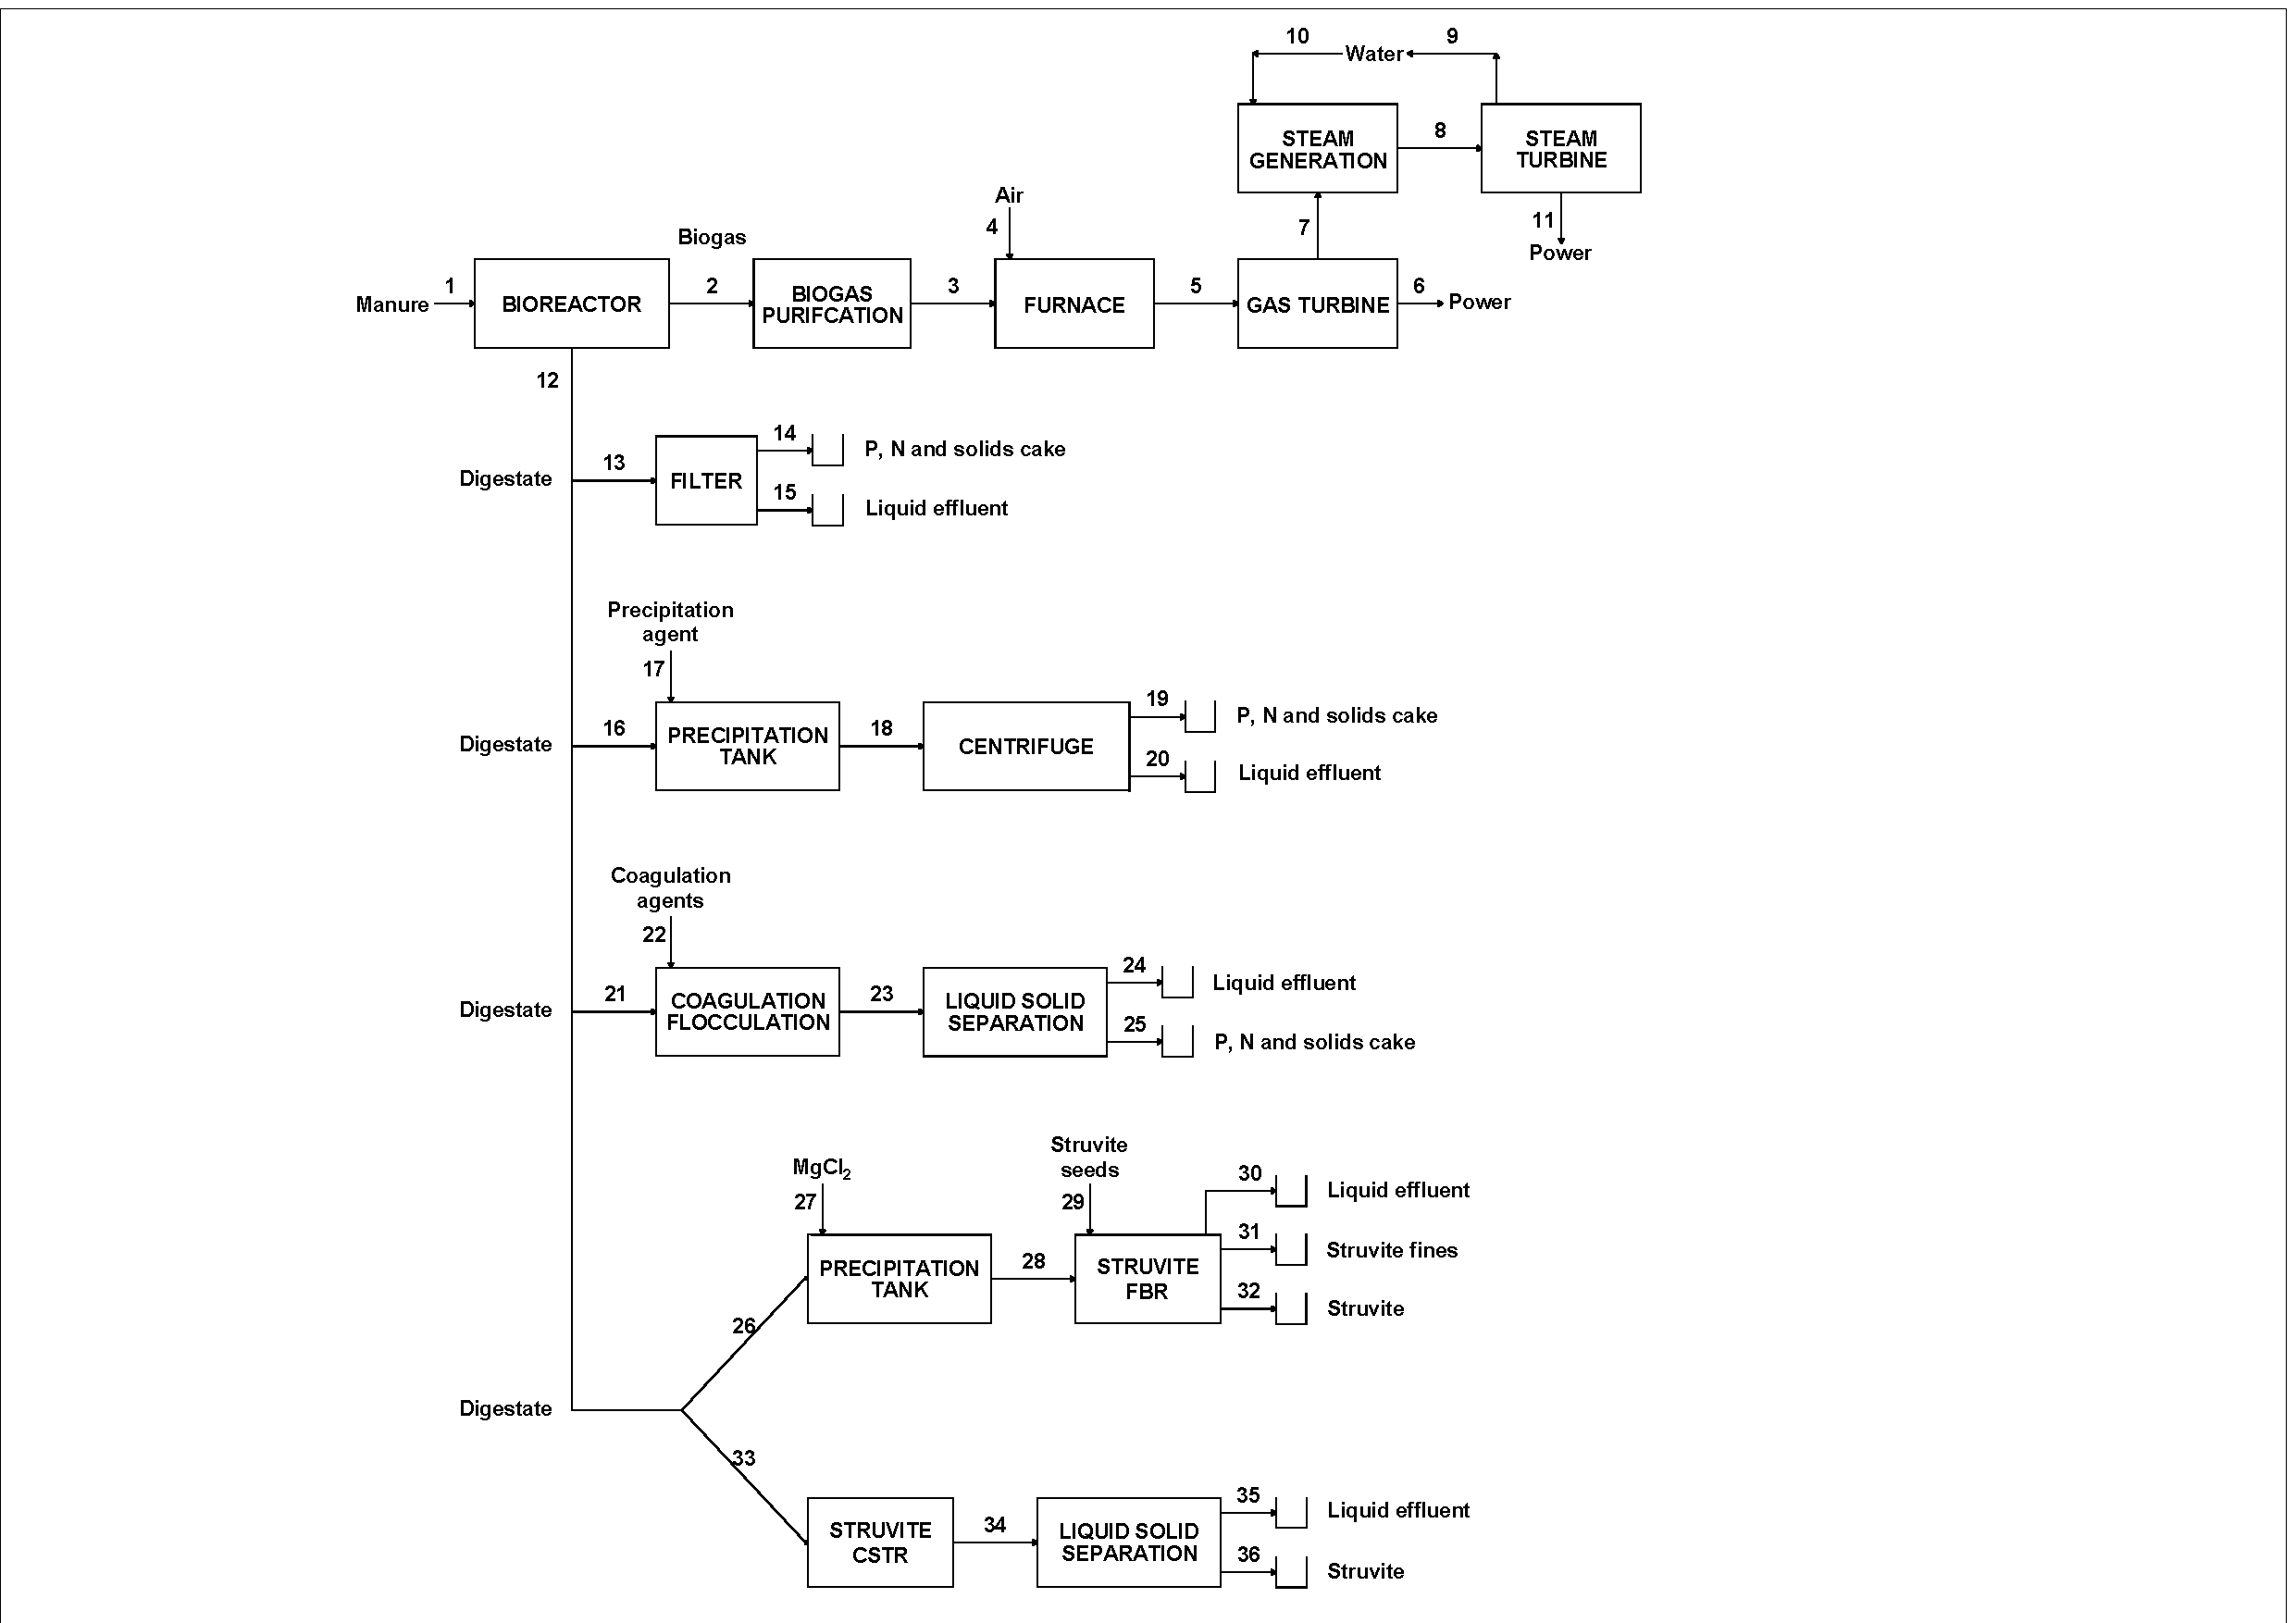
\includegraphics[width=1\linewidth, trim={6.5cm 0.1cm 11.5cm 0.3cm},clip]{gfx/Chapter2/superstructure3bloquesCOMPATIBILIDAD-Layout3.pdf} 
	\caption{Flowsheet for nutrient recovery and power production.}
	\label{fig:Flowsheet}
\end{figure}

The biomass together with water and nutrients (manure slurry) are fed to a bioreactor through stream 1, where the mixture is anaerobically digested to produce biogas and a decomposed substrate (digestate). The biogas, composed of methane, carbon dioxide, nitrogen, hydrogen sulfide, ammonia and moisture leaves the bioreactor through stream 2, and it is then sent to the purification section to remove H\textsubscript{2}S in a fixed-bed reactor and to eliminate CO\textsubscript{2} and traces of NH\textsubscript{3} in a second step by using a pressure swing adsorption (PSA) system. The purified biogas (stream 3) is used in a Brayton cycle, modelled as a furnace and an expansion, producing power. Air is fed via stream 4 and the exhaust gases (stream 7) are fed to a regenerative Rankine cycle, where it produces high pressure overheated steam extracted in stream 8. This overheated steam is fed to a steam turbine, where it is expanded to produce power. The exhaust steam from the turbine is recovered in stream 9 and reused in the Rankine cycle through stream 10. Between streams 9 and 10 hot flue gases from the gas turbine reheat and produced overheated steam from the recycled water \citep{Leon}.

The digestate is released from the digester through stream 12, and it can be processed through a number of technologies to remove nitrogen and phosphorous. We consider filtration, centrifugation, coagulation, and struvite production using either a fluidized bed reactor (FBR) or a continuous stirred tank reactor (CSTR). These technologies are described in detail in Section \ref{section:DigestateConditioning}.

Four manure types have been considered as raw material for the process: cattle, pig, poultry and sheep manure. Table \ref{table:techs_descriptionPaper1} shows the composition and properties of each type of manure.

\begin{table}[]
	\centering
	\caption{Manure composition and properties \protect\citep{kowalski2013changes, Lorimor2004, AlSeadi2008, martins2009biogas}.}
	\label{table:techs_descriptionPaper1}
	\resizebox{\columnwidth}{!}{
	\begin{tabular}{@{}ccccccccccccccc@{}}
		\toprule
		\multirow{2}{*}{\begin{tabular}[c]{@{}c@{}}Manure/\\ element\end{tabular}} & \multicolumn{2}{c}{\begin{tabular}[c]{@{}c@{}}Dry matter\\ (\% wt)\end{tabular}} & \multicolumn{2}{c}{\begin{tabular}[c]{@{}c@{}}N\\ (\% dry mass)\end{tabular}} & \multicolumn{2}{c}{\begin{tabular}[c]{@{}c@{}}P\\ (\% dry mass)\end{tabular}} & \multicolumn{2}{c}{\begin{tabular}[c]{@{}c@{}}K\\ (\% dry mass)\end{tabular}} & \multicolumn{2}{c}{\begin{tabular}[c]{@{}c@{}}VS\\ (\% dry mass)\end{tabular}} & \multicolumn{2}{c}{\begin{tabular}[c]{@{}c@{}}V\textsubscript{biogas}\\ $\left(\frac{\text{m\textsuperscript{3}\textsubscript{gas}}}{\text{kg\textsubscript{VS}}}\right)$\end{tabular}} & \multicolumn{2}{c}{\begin{tabular}[c]{@{}c@{}}Density\\ $\left(\frac{\text{kg}}{\text{m\textsuperscript{3}}}\right)$\end{tabular}} \\ \cmidrule(l){2-3} \cmidrule(l){4-5} \cmidrule(l){6-7} \cmidrule(l){8-9} \cmidrule(l){10-11} \cmidrule(l){12-13}
		& Max                                     & Min                                    & Max                                   & Min                                   & Max                                   & Min                                   & Max                                   & Min                                   & Max                                    & Min                                   & Max                                      & Min                                     &                                          &                                   \\ \midrule
		Cattle                                                                     & 10                                      & 2                                      & 8                                     & 4.7                                   & 1.3                                   & 0.8                                   & 10                                    & 3.3                                   & 0.8                                    & 0.8                                   & 0.3                                      & 0.2                                     & 1041.2                                   &                                   \\
		Pig                                                                        & 6                                       & 2                                      & 15                                    & 13                                    & 2.2                                   & 1.9                                   & 8.3                                   & 3.9                                   & 0.8                                    & 0.7                                   & 0.5                                      & 0.25                                    & 1000.0                                   &                                   \\
		Poultry                                                                    & 60                                      & 30                                     & 5.4                                   & 5.4                                   & 1.7                                   & 1.7                                   & 1.2                                   & 2.3                                   & 0.8                                    & 0.8                                   & 0.6                                      & 0.35                                    & 1009.2                                   &                                   \\
		Sheep                                                                      & 28                                      & 28                                     & 2.9                                   & 2.9                                   & 0.78                                  & 0.78                                  & 2.9                                   & 2.9                                   & 0.8                                    & 0.8                                   & 0.61                                     & 0.37                                    & 1009.2                                   &                                   \\ \bottomrule
	\end{tabular}
	}
\end{table}

\begin{table}[]
	\centering
	\caption{Set of components.}
	\label{table:SetComponents}
	\resizebox{\columnwidth}{!}{
		\begin{tabular}{@{}cccccccc@{}}
			\toprule
			\begin{tabular}[c]{@{}c@{}}Number of \\ component\end{tabular} & Component & \begin{tabular}[c]{@{}c@{}}Number of \\ component\end{tabular} & Component      & \begin{tabular}[c]{@{}c@{}}Number of \\ component\end{tabular} & Component      & \begin{tabular}[c]{@{}c@{}}Number of \\ component\end{tabular} & Component      \\ \midrule
			1                    & Wa        & 12                   & O              & 23                   & K\textsubscript{2}O            & 34                   & Cl             \\
			2                    & CO\textsubscript{2}       & 13                   & N              & 24                   & CaCO\textsubscript{3}          & 35                   & Struvite       \\
			3                    & CO        & 14                   & Norg           & 25                   & FeCl\textsubscript{3}          & 36                   & K-Struvite      \\
			4                    & O\textsubscript{2}        & 15                   & P              & 26                   & Antifoam       & 37                   & MgCl\textsubscript{2} (CSTR)     \\
			5                    & N\textsubscript{2}        & 16                   & K              & 27                   & Fe\textsubscript{2}(SO\textsubscript{4})\textsubscript{3}      & 38                   & NaOH (CSTR)      \\
			6                    & H\textsubscript{2}S      & 17                   & S              & 28                   & Al\textsubscript{2}(SO\textsubscript{4})\textsubscript{3}      & 39                   & Mg (CSTR)        \\
			7                    & NH\textsubscript{3}       & 18                   & Rest           & 29                   & AlCl\textsubscript{3}          & 40                   & Cl (CSTR)        \\
			8                    & CH\textsubscript{4}       & 19                   & Cattle slurry  & 30                   & MgCl\textsubscript{2}          & 41                   & Struvite (CSTR)  \\
			9                    & SO\textsubscript{2}       & 20                   & Pig slurry     & 31                   & NaOH           & 42                   & K-Struvite (CSTR) \\
			10                   & C         & 21                   & Poultry slurry & 32                   & Struvite seeds & 43                   & FeCl\textsubscript{3} Coag     \\
			11                   & H         & 22                   & P\textsubscript{2}O\textsubscript{5}          & 33                   & Mg             &                      &     \\          
		\bottomrule
		\end{tabular}
	}
\end{table}


\section{Modelling issues} \label{section:ModellingIssues}
We evaluate the performance of the different unit operations in the process by using detailed models that comprise mass and energy balances, thermodynamics, chemical and vapor–liquid equilibria, and product yield calculations. The global process model comprises total mass flows, component mass flows, component mass fractions, temperatures and pressures of the streams in the process network. The components that are considered in our calculations belong to the set shown in Table \ref{table:SetComponents}.

In the following subsections, we briefly present the main equations used to characterize the operation of the different units. For the sake of brevity, simpler balances based on removal efficiency or stoichiometry and equations connecting units are omitted. The power production system is described in detail in previous work \citep{Leon} and we thus only provide a brief description.

The cost estimation for the alternatives and for the entire process is based on the estimation of the unit costs from different sources using the factorial method. From the units cost, the facility cost is estimated using the coefficients in \citet{sinnott1999chemical}, so that the total physical plant cost involving equipment erection, piping instrumentation, electrical, buildings, utilities, storage, site development, and ancillary buildings is 3.15 times the total equipment cost for processes which use fluids and solids. On the other hand, the fixed cost, which includes design and engineering, contractor’s fees, and contingency items is determined as 1.4 times the total physical plant cost for the fluid and solid processes. In the subsequent cost estimation procedures these parameters are denoted as $f_i$ for the total physical plant parameter and $f_j$ for the fixed cost parameter.


\subsection{Biogas production} \label{section:BiogasProduction}
AD is a complex microbiological process that decomposes organic matter in the absence of oxygen. It produces a gas mixture following hydrolysis, acidogenesis, acetogenesis, and methanogenesis steps, consisting mainly of methane and carbon dioxide (biogas), and decomposed substrate (digestate). The anaerobic reactor is modeled using mass balances of the species involved in the production of biogas and digestate. Inorganic nitrogen, organic nitrogen, sulfur, carbon, and phosphorus balances are formulated by using the composition of volatile solids in manure, see Table \ref{table:techs_descriptionPaper1} \citep{kowalski2013changes, Lorimor2004, AlSeadi2008, martins2009biogas}. Typical bounds for the biogas composition are provided. The reactor operates at 55 \textdegree C. We refer the reader to the Supplementary Material and \citet{Leon} for details on the modelling of the digester.

\subsection{Biogas purification} \label{section:BiogasPurification}
This system consists of a number of stages to remove H\textsubscript{2}S, CO\textsubscript{2} and NH\textsubscript{3}. Here we highlight some basics about the operation of these stages. For further details we refer the reader to previous work \citep{Leon}.

The removal of H\textsubscript{2}S is carried out in a bed of Fe\textsubscript{2}O\textsubscript{3}, that operates at 25–50 \textdegree C producing Fe\textsubscript{2}S\textsubscript{3}. The regeneration of the bed
uses oxygen to produce elemental sulfur and Fe\textsubscript{2}O\textsubscript{3}.

CO\textsubscript{2} is adsorbed using a packed bed of zeolite 5A. The typical operating conditions for PSA systems are low temperature (25 \textdegree C) and moderate pressure (4.5 bar). The recovery of the PSA system is assumed to be 100\% for NH\textsubscript{3} and H\textsubscript{2}O (because of their low total quantities in the biogas, in general), 95\% for CO\textsubscript{2} , and 0\% for all other gas of the mixture.

In both cases the system is modelled as two beds in parallel so that one bed is in adsorption mode while the second one is in regeneration mode, to allow for continuous operation of the plant. Further details can be found in the Supplementary Material.

\subsection{Electricity generation} \label{section:ElectricityGeneration}
We consider two stages for the generation of power. The initial one consists of the use of a gas turbine, a common alternative for using any gas fuel. However, the flue gas that exits the gas turbine is at high temperature. We can either produce steam as a utility or use that steam within a regenerative Rankine cycle to enhance the production of power. The details for the process appear in \citet{Leon} or in the Supplementary Material.

\subsubsection{Brayton cycle}  \label{section:BraytonCycle}
We model the Brayton cycle as a double-stage compression system (one for the air and one for the fuel) with intercooling with variable operating pressure for the gas turbine. The compression is assumed to be polytropic with a coefficient equal to 1.4 and an efficiency of 85\% \citep{Moran2003}.

The combustion of methane from the biogas is assumed to be adiabatic, heating up the mixture. We consider the combustion chamber as an adiabatic furnace. We use an excess of 20\% of air with respect to the stoichiometry and 100\% conversion of the reaction:
\begin{align}
	& \text{CH}_4 + 2\text{O}_2 \rightarrow \text{CO}_2 + 2\text{H}_2 \text{O}
\end{align}

The hot flue gas is expanded in the gas turbine to generate power and the expansion is assumed polytropic. In this case, a value of 1.3 is used based on an offline simulation using CHEMCAD\textsuperscript{\textregistered}, with an efficiency of 85\% \citep{Moran2003}. Finally, the exhaust gas is cooled down and used to generate high-pressure steam to be fed to the Rankine cycle.

\subsubsection{Rankine cycle} \label{section:RankineCycle}
We use the hot flue gas from the turbine to generate steam following a scheme that consists of using the hot gas in the order that follows. First, the hot flue gas is used for the superheating stage of the steam that is to be fed to the turbine. Next, the hot gas is used in the regenerative stage of the Rankine cycle, reheating the steam from the expansion of the high pressure turbine. Subsequently, the flue gas is used in the evaporation and preheating of the condensed water, see Figure \ref{fig:Flowsheet}. The details of the modelling of the Rankine cycle can be seen in \citet{martin2013optimal}. We assume an isentropic efficiency of 0.9 for each expansion.

\subsection{Digestate conditioning} \label{section:DigestateConditioning}
Four different alternatives are considered to process the digestate including filtration, centrifugation, coagulation, and struvite production. For struvite production, the performance of fluidized bed reactors (FBR) and stirred tanks reactors (CSTR) systems is compared. For filtration, centrifugation, and coagulation technologies, nutrients output is a cake composed of different solids and nutrients, with a complex composition. The credit that we can get from the cake has been estimated based on the amount of nutrients contained. The prices for the nutrients (N, P and K) are assumed as follows: 0.45 \texteuro/kg for N, 0.24 \texteuro/kg for K and 0.32 \texteuro/kg for P \citep{hernandez2017bio}.

\subsubsection{Filtration}
Filtration is a low-cost technology that is appropriate for small installations where the amount of P to be removed is moderate. This technology consists of a filter that contains a reactive medium to help remove phosphorus. P removal using reactive filtration takes place through various mechanisms depending on the characteristics of the filter media. For instance, filter media made of compounds rich in cations under basic environments (usually containing calcium silicates at pH values above 9) form orthophosphate precipitates in the form of calcium phosphates, principally as hydroxyapatite \citep{pratt2012biologically}. Metallurgical slag captures P by adsorption over metal at pH close to 7 \citep{pratt2012biologically}. In this work we consider the use of five different types of filter media. Among them, we have studied wollastonite as a filter media rich in alkaline calcium silicates, dolomite Polonite\textsuperscript{\textregistered} as calcium carbonate based components, and Filtra P as calcium hydroxide based product \citep{osterberg2012removal, vohla2011filter}. For the metallurgical slag, we have considered the blast furnace slag described by \citet{cucarella2008effect}. These filters are used in wastewater treatment facilities \citep{gustafsson2008phosphate} and further analysis can be found in \citet{shilton2006phosphorus}. Details on Ca-rich filters can be found in \citet{koiv2010phosphorus}. The removal yield of P and N for the different filter media is shown in Table 3. It is possible to combine this filter medium with nitrogen-philic filters to simultaneously remove nitrogen and phosphorous. An advantage of this technology is that the cake produced can be used as soil fertilizer \citep{hylander2006phosphorus}. The removal yield of nitrogen for Filtra P\textsuperscript{\textregistered} has been considered similar to the limestone nitrogen removal yield, as Filtra P\textsuperscript{\textregistered} is a limestone derived product.

The model for the filtration is based on the removal efficiency per filter media, see Fig. \ref{fig:FilterScheme}. It has been considered that materials such as total solids, carbon and potassium are forming solid compounds, so they will be retained by the filter media, Eqs. \ref{eq:Eq4}–\ref{eq:Eq7}.
\begin{figure}[h!]
	\centering
	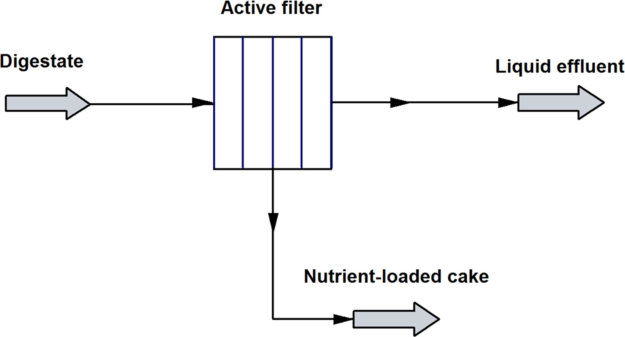
\includegraphics[width=0.6\linewidth, trim={0cm 0cm 0cm 0cm},clip]{gfx/Chapter2/Fig2.pdf} 
	\caption{Scheme of the filter.}
	\label{fig:FilterScheme}
\end{figure}

\begin{equation}
	\begin{aligned}
		& F_i^{{cake}} \ge F_i^{{in}} \cdot \eta _i^{j} - M\cdot \left(1 - {y^j}\right) \\
		& {i} \in \left\{ \text{P, N} \right\} \\
		& j \in \left\{ {{\text{filter media}}} \right\} \label{eq:Eq2}
	\end{aligned}
\end{equation}

\begin{table}[h]
	\centering
	\caption{Recovered P and N yield for different filter media..}
	\label{table:Table3}
%	\resizebox{\columnwidth}{!}{
	\begin{threeparttable}
		\begin{tabular}{@{}ccc@{}}
			\toprule
			Media/nutrient & P (\% recovered) & N (\% recovered) \\ \midrule
			Polonite       & 96.7\textsuperscript{a}           & 18.0\textsuperscript{c}            \\
			Filtra P       & 98.2\textsuperscript{a}           & 50.0\textsuperscript{e}            \\
			Wollastonite   & 51.1\textsuperscript{a}           & 70.0\textsuperscript{d}            \\
			Dolomite       & 44.0\textsuperscript{b}           & 50.0\textsuperscript{e}            \\
			Metal slag     & 85.6\textsuperscript{a}           & 67.0\textsuperscript{f}            \\ \bottomrule
		\end{tabular}
%	}
	\begin{tablenotes}
		\footnotesize
		\item {a}: \citet{gustafsson2008phosphate}
		\item {b}: \citet{pant2001phosphorus}
		\item {c}: \citet{kietlinska2005evaluation}
		\item {d}: \citet{lind2000nutrient}
		\item {e}: \citet{aziz2004removal}
		\item {f}: \citet{yang2009converter}
	\end{tablenotes}
	\end{threeparttable}
\end{table}

\begin{align}
	\sum {{y}}^{{j}} { = 1} \label{eq:Eq3}
\end{align}

\begin{align}
	F_i^{{liquid \ effluent}} = F_i^{{in}} - F_{{i}}^{{cake}} \label{eq:Eq4}
\end{align}
%
\begin{align}
	F_k^{{cake}} = F_k^{{in}}; \ {k} \in \left\{ \text{TS, C ,K} \right\} \label{eq:Eq5}
\end{align}

\begin{align}
	F_{Wa}^{{cake}} = \left( {F_{TS}^{{cake}} + \sum\limits_i {F_i^{{cake}}} } \right) \cdot \frac{C_{Wa}^{cake}}{1 - C_{Wa}^{{cake}}} \label{eq:Eq6}
\end{align}
%%

\begin{align}
	F_{Wa}^{{{liquid \ effluent}}} = F_{Wa}^{{in}} - F_{Wa}^{{cake}} \label{eq:Eq7}
\end{align}

To select among the five filter media, we use a Big M formulation to select one of them assigning a binary variable $y^{\text{filter media}}$ for each filter media, Eqs. \ref{eq:Eq2} and \ref{eq:Eq3}. This variable takes a value of 1 for the selected filter media and 0 for the rest, so that we are able to evaluate one filter media per time.

It is assumed that the cake obtained contains moisture with a value of 55\% in weight basis $\left(C_{Wa}^{cake}\right)$. The optimal filter media among the evaluated compounds is metal slag \citep{li2015study}.

The cost of each alternative has been estimated according to the number of filters, which depends on the maximum flow they can process. The maximum flow per filter unit, $F_{max}^{{filter}}$, is 1,300 ft\textsuperscript{3}/min \citep{loh2002process}. To design the filter units we have taken the minimum value between the flow provided by mass balances and the maximum flow allowed per filter, Eqs. \ref{eq:Eq8}–\ref{eq:Eq10}.

\begin{align}
	F\left( {\frac{\text{ft}^3}{\text{min}}} \right) = \frac{{{F_{in}}}}{{{\rho _{{digestate}}}}} \label{eq:Eq8}
\end{align}

\begin{align}
	{n}_{{filters}} \ge \frac{F_{total}^{{filter}}}{F_{{max}}^{{filter}}} 	\label{eq:Eq9}
\end{align}

\begin{align}
	F_{design}^{{filter}}\left( {\frac{\text{ft}^3}{\text{min}}} \right) = \min \left( {F_{max}^{{filter}},F_{total}^{{filter}}} \right) \label{eq:Eq10}
\end{align}

In fact, since the maximum flow for a cartridge filter is 1,300 ft\textsuperscript{3}/min, for this facility the number of filters considered in this work will always be one and the design flow is equal to the flow provided by mass balances.

The correlation used to calculate the filter cost, Eq. \ref{eq:Eq11}, is obtained from data reported in \citet{loh2002process}. This correlation provides the price in 1998 dollars, so we use the Chemical Engineering Index to update it.

\begin{align}
	FC_{filtration}\left( \text{USD}  \right) = 4.7436\cdot F_{design}^{{filter}} + 807.6923 \label{eq:Eq11}
\end{align}

The operating cost is estimated using a simple correlation, Eq. \ref{eq:Eq14}, where we assume that the utilities contribute 20\% of the total \citep{vian1975pronostico}. The other economical contributions considered are chemicals, estimated as in Eq. \ref{eq:Eq12}, labour, as per Eq. \ref{eq:Eq13}, and the contribution of the investment cost of the units given by Eqs. \ref{eq:Eq10} and \ref{eq:Eq11}. The filter media are considered as chemicals that will be replaces annually.

\begin{align}
	{ChemC}_{filtration}\left(\frac{\text{EUR}}{\text{year}}\right) = 	\frac{F_{P}^{in} \cdot 3600 \cdot h \cdot d}{\frac{kg_P}{kg_{{filter \ media}}}} \cdot {Price}_{{filter \ media}} \label{eq:Eq12}
\end{align}

In Eq. \ref{eq:Eq12}, $kg_{{filter \ media}}$ are calculated as the P content in the inlet stream divided by the filter media P adsorption capacity.

\begin{align}
	& {{Labour \ cost}}\left( \frac{\text{EUR}}{\text{year}} \right) = \label{eq:Eq13} \\
	& \left( 61.33\cdot F_P^{recovered} \cdot 3.6\cdot{{{h}^{\left( { - 0.82} \right)}}} \right) \cdot \left( {F_P^{recovered} \cdot 3.6 \cdot h \cdot d} \right) \cdot \left( {\frac{{Salary}}{{h \cdot d}}} \right)\cdot{n_{OP}} \nonumber 
\end{align}

The number of operations considered, $n_{OP}$ , is equal to 1.

\begin{align}
	&{{Operating \ cost}}\left( \frac{\text{EUR}}{\text{year}} \right) = \label{eq:Eq14}\\ 
	&\frac{{{{ChemC}} + 1.5\cdot{{Labour \ cost}} + 0.3 \cdot Fixed \ Cost\cdot{f_i}\cdot{f_j}}}{{(1 - Utilities)}} \nonumber 
\end{align}

Finally the credit obtained from the cake is computed as the weighted sum of each nutrient value, Eq. \ref{eq:Eq15}, \citep{hernandez2017bio}, and the benefits (or losses) are computed as the difference between the credit obtained from the cake and the operating costs of the facility, Eq. \ref{eq:Eq16}.

\begin{align}
	& Cost_{cake} \left( \frac{\text{EUR}}{\text{year}} \right) = \label{eq:Eq15} \\ 
	& \left( {F_P^{recovered}\cdot{Price_P} + F_N^{recovered}\cdot{Price}_N} + F_K^{recovered}\cdot{Price_K} \right) \nonumber \\
	& \cdot 3600\cdot h \cdot d \nonumber
\end{align}

\begin{align}
	{{Benefits}}_{Filtration} \left(\frac{\text{EUR}}{\text{year}}  \right) = Cost_{cake} - {{Operating \  cost}} \label{eq:Eq16}
\end{align}

\subsubsection{Coagulation}
\begin{figure}[h!]
	\centering
	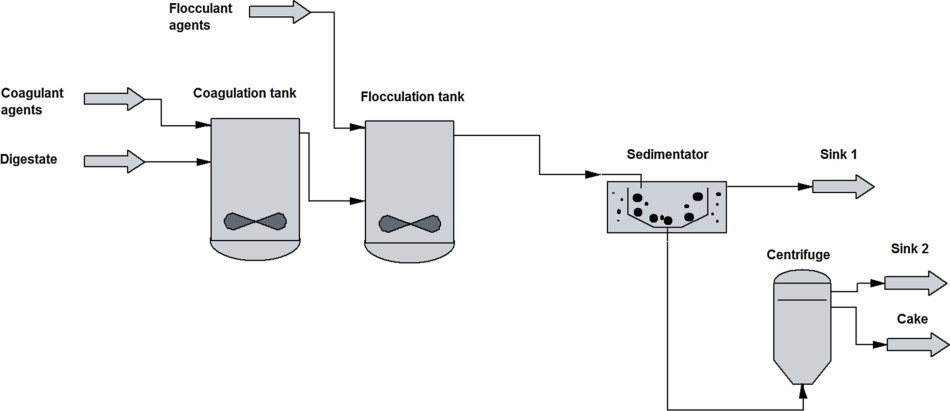
\includegraphics[width=1\linewidth, trim={0cm 0cm 0cm 0cm},clip]{gfx/Chapter2/Fig3.pdf} 
	\caption{Scheme of the coagulation process.}
	\label{fig:CoagScheme}
\end{figure}

Coagulation is a chemical treatment to process the digestate. The goal of this process is to destabilize colloidal suspensions by reducing the attractive forces, followed by a flocculation process to form flocs from the previously destabilized colloids and to subsequently precipitate them. The nutrients are then recovered with other sedimented solids by clarification. Both N and P can be removed from the influent through coagulation–flocculation, where phosphorus is removed primarily in the form of metal hydroxides, which is the dominant process at typical plant pH values \citep{szabo2008significance}. Nitrogen elimination is related to the removal of the colloidal matter \citep{aguilar2002nutrient}. Different coagulation agents are considered aiming at selecting the optimal one: FeCl\textsubscript{3}, Fe\textsubscript{2}(SO\textsubscript{4})\textsubscript{3}, Al\textsubscript{2}(SO\textsubscript{4})\textsubscript{3}, and AlCl\textsubscript{3}. The flowsheet for the process of coagulation is presented in Fig. \ref{fig:CoagScheme}.

The removal efficiency achieved is similar for the different coagulant agents, with values up to 99\% for phosphorus and 57\% for nitrogen \citep{aguilar2002nutrient}. The main variables which influence the coagulation–flocculation process are the initial ratio of metal to phosphorus, pH, and chemical oxygen demand (COD). The initial metal-phosphorus molar ratio must be between 1.5 and 2.0, and the recommended pH range is from 5.5 to 7. COD has a negative impact on the removal efficiency when its value is increased \citep{szabo2008significance}.

To determine the amount of coagulant agent to be added to the system, it has been considered that a metal/phosphorus molar ratio of 1.75 must be achieved \citep{szabo2008significance}. Given the relationship between the P in the raw material stream, the metal added, and the metal concentration in the commercial presentation of the coagulant agent, we are able to compute the coagulant agent amount that should be added. In the coagulation and flocculation tanks the flocs are formed and nutrients are recovered in the sediment together with coagulation agents and organic solids contained in the raw material. In the decanter, it has been considered that the stream with solids has a water content of 50\% $\left(C^{sedimentator}_{Wa}\right)$ \citep{williams2011digestates} and the water content of the centrifuge outlet solids stream is 60\% $\left(C^{centrifuge}_{Wa}\right)$ \citep{wakeman2007separation}.

Other elements present in the digestate, such as total solids, carbon, and potassium are assumed to be present in the solid forming compounds that sediment. Thus, they are among species that constitute the cake. Taking into account the elements mentioned above mass balances have been formulated with the corresponding removal ratios. To select and evaluate the different coagulant agents, the problem has been modelled using a mixed-integer nonlinear programming (MINLP) formulation with Big-M constraints, Eqs. \ref{eq:Eq17} and \ref{eq:Eq18}.

\begin{align}
	& F_j^{{{coag \ tank}}} \ge \frac{F_P^{in}}{MW_P} \cdot MeP_{ratio} \cdot \frac{MW_j}{C_{Me}} - M \cdot \left(1 - {y^j}\right) \label{eq:Eq17} \\
	& {j} \in \left\{ \text{coagulant agents} \right\} \nonumber
\end{align}

\begin{align}
	\sum {{{{y}}^j}} = 1 \label{eq:Eq18}
\end{align}

where $MeP$ is the metal/phosphorus ratio and M is a large value to formulate the Big-M constraint to select and evaluate the different coagulant agents. Mass balances are computed using Eqs. \ref{eq:Eq19}–\ref{eq:Eq28}.

\begin{align}
	& F_j^{{{coag \ tank}}} = F_j^{{{floc \ tank}}} = F_j^{{{sedimentator}}} = F_j^{{{centrifuge}}} = F_j^{{{cake}}} \label{eq:Eq19}\\
	& j \in \left\{ \text{coagulants} \right\} \nonumber
\end{align}

\begin{align}
	& F_i^{in} = F_i^{{{coag \ tank}}} = F_i^{{{floc \ tank}}} = F_i^{{{sedimentator}}} \label{eq:Eq20} \\
	& {i} \in \left\{ \text{P, N} \right\} \nonumber
\end{align}

\begin{align}
	F_i^{cake} = F_i^{centrifuge} = F_i^{{{sedimentator}}} \cdot \eta_i^j \label{eq:Eq21}
\end{align}

\begin{align}
	F_i^{{{sink1}}} = F_i^{{{sedimentator}}} - F_i^{{{centrifuge}}} \label{eq:Eq22}
\end{align}

\begin{align}
	& F_k^{in} = F_k^{{{coag \ tank}}} = F_k^{{{floc \ tank}}} = F_k^{{{sedimentator}}} = F_k^{{{centrifuge}}} = {{F}}_{{k}}^{{{cake}}} \label{eq:Eq23} \\
	& {{k}} \in \left\{ \text{TS, C, K} \right\} \nonumber
\end{align}

\begin{align}
	F_{Wa}^{in} = F_{Wa}^{{{coag \ tank}}} = F_{Wa}^{{{floc \ tank}}} = F_{Wa}^{{{sedimentator}}} \label{eq:Eq24}
\end{align}

\begin{align}
	& {F}_{{Wa}}^{centrifuge} = \label{eq:Eq25} \\
	& \left( {{F}_{TS}^{centrifuge} + \sum\limits_i {{F}_i^{centrifuge} + \sum\limits_j {F}_j^{centrifuge}} }  \right) \cdot \frac{{C_{Wa}^{sedimentator}}}{1 - C_{Wa}^{centrifuge}} \nonumber
\end{align}

\begin{align}
	{F}_{Wa}^{sink1} = F_{Wa}^{sedimentator} - {F}_{Wa}^{centrifuge} \label{eq:Eq26}
\end{align}

\begin{align}
	{F}_{Wa}^{cake} = \left( {F}_{TS}^{cake} + \sum\limits_i {F_i^{cake} + \sum\limits_j {F}_j^{cake}}  \right) \cdot \frac{{C_{Wa}^{centrifuge}}}{{1 - C_{Wa}^{centrifuge}}} \label{eq:Eq27}
\end{align}

\begin{align}
	{F}_{Wa}^{sink2} = F_{Wa}^{centrifuge} - F_{Wa}^{cake} \label{eq:Eq28}
\end{align}

The estimation of the size and cost of both the coagulation and flocculation tanks has been carried out using a correlation developed by \citet{almena2016technoeconomic} as a function of the weight of the vessels. To simplify the mass balances it is considered that the volume provided by the coagulant agents is negligible with respect to the processed stream of the digestate. The vessel size is computed from the residence time. The hydraulic retention time considered in the coagulation tank is 4 min \citep{zhou2008enhanced}. The vessel size is computed from the residence time, Eq. \ref{eq:Eq29}. Using these data, the diameter and length are computed using rules of thumb, Eqs. \ref{eq:Eq30} and \ref{eq:Eq31}. Finally, a correlation for the thickness as a function of the diameters allows determining the mass of metal required for the vessel and its weight, Eqs. \ref{eq:Eq32} and \ref{eq:Eq33}. Vessel cost estimation is provided by Eq. \ref{eq:Eq34}.

\begin{align}
	{V}_{Coag \ tank}\left( \text{m}^{3} \right) = HR{T_{Coag \ tank}} \cdot \frac{F_{digestate}^{in}}{\rho_{digestate}} \label{eq:Eq29}
\end{align}

\begin{align}
	{D_{Coag \ tank}} \left( \text{m} \right) = \left( \frac{6 \cdot{V}_{Coag \ tank}}{7 \cdot \pi} \right)^{1/3} \label{eq:Eq30}
\end{align}

\begin{align}
	{L_{{{Coag \ tank}}}}\left( m \right) = 4\cdot{D_{Coag \ tank}} \label{eq:Eq31}
\end{align}

\begin{align}
	{e_{Coag \ tank}}\left( \text{m} \right) = 0.0023 + 0.003\cdot{D_{{{Coag \ tank}}}} \label{eq:Eq32}
\end{align}

\begin{align}
	& {W_{Coag \ tank}}\left( \text{kg} \right) = {\rho_{SS316}}\cdot \label{eq:Eq33} \\
	& \Bigg[ \pi \cdot \left( {{{\left( \frac{{{D_{Coag tank}}}}{2} + {e_{Coag \ tank}} \right)}^2} - {{\left( \frac{{{D_{Prec \ tank}}}}{2} \right)}^2}} \right)\cdot{L_{Coag \ tank}} + \nonumber \\ 
	& \frac{4}{3} \cdot \pi \cdot \left( \left( \frac{D_{Coag \ tank}}{2} + {e_{Coag \ tank}} \right)^3 - \left( \frac{D_{Coag \ tank}}{2} \right)^3 \right) \Bigg] \nonumber
\end{align}

\begin{align}
	{Cost}_{Vessel} \left( \text{USD} \right) = 6839.8 \cdot {V}_{Coag \ tank}{\left( {\text{m}^{3}} \right)^{0.65}} \label{eq:Eq34}
\end{align}

To estimate the power consumed by the agitator, Eq. \ref{eq:Eq35}, rules of thumb have been used; where the specific power consumed, $\kappa_{agitator}$, is tabulated in \citet{walas1988chemical}. For our slurries a value of $\kappa_{agitator}$ equal to 10 HP per 1000 US gallons is the most appropriate.

\begin{align}
	P_{Agitator}\left( \text{HP} \right) = V_{Coag \ tank} \left( {\text{US gallon}} \right) \cdot \frac{\kappa_{agitator}}{1000} \label{eq:Eq35}
\end{align}

The agitator cost is also estimated using a correlation from \citet{walas1988chemical}, Eq. \ref{eq:Eq36}. For cost estimation purposes we have considered stainless steel 316 as construction material and a dual impeller operating at speed between 56 and 100 rpm depending on the tanks size. With these considerations the values for $a$, $b$ and $c$ are 8.8200, 0.1235 and 0.0818 respectively \citep{walas1988chemical}. This correlation provides the cost in 1985 dollars, so it is necessary to update the result using the Chemical Engineering Index as before.

\begin{align}
	Cost_{Agitator} \left( \text{USD}_{1985}  \right) = {e^{a + b \cdot {\text{ln}}\left( {{P_{agitator}}\left( \text{HP} \right)} \right) + c \cdot {\left[ \text{ln}\left( {P_{agitator}\left( \text{HP} \right)} \right) \right] }^2}} \label{eq:Eq36}
\end{align}

The total cost of the coagulation tank is equal to the sum of the vessel cost and the agitator cost, Eq. \ref{eq:Eq37}.

\begin{align}
	{Cost}_{Coag \ tank} = Cost_{Vessel} + Cost_{Agitator} \label{eq:Eq37}
\end{align}

The flocculation tank is designed similarly to that of the coagulation, using Eqs. \ref{eq:Eq29}–\ref{eq:Eq37}. For this step the hydraulic retention time is 25 min \citep{zhou2008enhanced}.

The decanter is assumed to be circular because of its lower operating and maintenance costs. The area, Eq. \ref{eq:Eq38}, is computed using the parameter $A_{specific}$, which is the specific clarifier area in m\textsuperscript{2} per ton of inlet flow per day \citep{wef2005wef}. The typical value, 10 m\textsuperscript{2}/(t/day), is taken from \citet{green2008perry}. The diameter of the clarifier, $D^{clarifier}$, is computed from the area value, Eq. \ref{eq:Eq39}.

\begin{align}
	{A}_{clarifier} \left( \text{m}^2 \right) = \frac{A_{specific} \cdot F_{digestate}^{in}\left( \frac{\text{m}^3}{\text{day}} \right)}{1000} \label{eq:Eq38}
\end{align}

\begin{align}
	D_{clarifier} \left( \text{m} \right) = \left( \frac{4 \cdot A_{clarifier}}{\pi} \right)^{1/2} \label{eq:Eq39}
\end{align}

The number of clarifiers is an integer value that is computed as the minimum integer from the ratio between the clarifier diameter calculated before and the maximum clarifier diameter, $D_{max}^{clarifier}$, Eq. \ref{eq:Eq40}. The maximum clarifier diameter value considered is 40 m \citep{green2008perry}.

\begin{align}
	{n}_{clarifiers} \ge \frac{D^{clarifier}}{D_{max}^{clarifier}} \label{eq:Eq40}
\end{align}

The diameter used in the final design will be the smallest between $D^{clarifier}$ and $D_{max}^{clarifier}$, Eq. \ref{eq:Eq41}.

\begin{align}
	D_{design}^{clarifier} \left( \text{m} \right) = \text{min}(D_{max}^{clarifier},D^{clarifier}) \label{eq:Eq41}
\end{align}

To model the minimization function and compute $D_{design}^{clarifier}$, the following smooth function approximation, given by Eq. \ref{eq:Eq42}, is used based on a previous work \citep{de2016characterization} to avoid discontinuities within the problem formulation.

\begin{align}
	D_{design}^{clarifier} \left( \text{m} \right) = \frac{D_{max}^{clarifier}}{1 + {e^{\left( -F_{digestate}^{in} + 0.342 \right) \cdot 2.718}}} \label{eq:Eq42}
\end{align}

The cost estimation correlation has been developed from the data in \citet{wef2005wef}, Eq. \ref{eq:Eq43}. It includes all the items involved in the operation of such an unit. The correlation must be updated to current prices using the Chemical Engineering Index.

\begin{align}
	Cost_{clarifier} \left( \text{USD}_{1979} \right) = \left( 13060 \cdot D_{design}^{clarifier} - 58763 \right) \cdot {n}_{clarifiers} \label{eq:Eq43}
\end{align}

Centrifuge sizing and costing is based on the data by \citet{green2008perry}. We assume pusher type with a maximum diameter of 1250 mm. The modelling equation for sizing is given in Eq. \ref{eq:Eq44}.

\begin{align}
	D_{Centrifuge}\left( \text{in} \right) = 0.3308 \cdot \frac{F_{digestate}^{in}}{1000}\cdot 3600 + 9.5092 \label{eq:Eq44}
\end{align}

The number of centrifuges is calculated taking into account the maximum centrifuge diameter, Eq. \ref{eq:Eq45}, and the diameter used in the final design will be the minimum value between $D^{centrifuge}$ and $D_{max}^{centrifuge}$, Eq. \ref{eq:Eq46}.

\begin{align}
	{n}_{centrifuges} \ge \frac{D^{centrifuge}}{D_{max}^{centrifuge}} \label{eq:Eq45}
\end{align}

\begin{align}
	D_{design}^{centrifuge} = \min \left( {D_{max}^{centrifuge}, D^{centrifuge}} \right) \label{eq:Eq46}
\end{align}

As in the clarifier, we develop a smooth approximation, Eq. \ref{eq:Eq47}, to compute the design diameter avoiding discontinuities as follows:

\begin{align}
	D_{design}^{centrifuge} = \frac{D_{max}^{centrifuge}}{1 + {e^{\left( { -F_{digestate}^{in} + 35.369} \right) \cdot 0.0395}}} \label{eq:Eq47}
\end{align}

The cost for the centrifuge is estimated based on the data by \citet{green2008perry} as a function of its diameter, Eq. \ref{eq:Eq48}. Since the cost correlation is based on 2004 values, the Chemical Engineering Index it used to update the equipment cost.

\begin{align}
	& Cost_{centrifuge}\left( \text{USD}_{2004}  \right) = \label{eq:Eq48} \\
	& \left( {10272 \cdot D_{design}^{centrifuge} - 24512} \right) \cdot {n}_{centrifuges} \nonumber
\end{align}

We estimate the operating cost of this system by accounting for the annualized equipment cost (fixed cost), chemicals and labor cost. A similar procedure as before is followed \citep{vian1975pronostico} but for the clarifier fixed costs as the correlation to estimate its costs already includes the operating cost, Eq. \ref{eq:Eq49}.

\begin{align}
	& FC_{coagulation} \left( \frac{ \text{EUR} }{\text{year}} \right) = \label{eq:Eq49}\\
	& \left( {Cost}_{Coag \ tank} + {Cost}_{Floc \ tank} + Cost_{centrifuge} \right) \cdot {f_i} \cdot {f_j} + Cost_{clarifier} \nonumber
\end{align}

The chemicals costs are estimated as Eq. \ref{eq:Eq50}.

\begin{align}
	& {ChemC}_{coagulation} \left( \frac{ \text{EUR} }{\text{year}} \right) = \label{eq:Eq50} \\
	& \big( F_{Fe_2 \left(SO_{4} \right)_3}^{in} \cdot Price_{Fe_2 \left( SO_{4} \right)_3} + F_{Al_{2} \left( SO_{4} \right)_3}^{in} \cdot Price_{Al_{2} \left( SO_{4} \right)_3} + \nonumber \\
	& F_{FeCl_{3}}^{in} \cdot Price_{FeCl_{3}} + F_{AlCl_{3}}^{in} \cdot Price_{AlCl_{3}} \big) \cdot 3600\cdot h \cdot d \nonumber
\end{align}

To estimate the price for the cake, as in the previous case, we assume the price of each of the nutrients contained (N, P, and K). The price for each nutrient is taken same as before. Thus, the cake price is computed as the weighted sum of each nutrient, as in Eq. \ref{eq:Eq15} \citep{hernandez2017bio}.

Finally, the economic benefits or losses of operating this system are calculated as the difference between the credit obtained from the cake and the operating costs of section of the facility, as in Eq. \ref{eq:Eq16}.

\subsubsection{Centrifugation}
Centrifugation is a pretreatment that separates solid and liquid phases and that can be used to recover nutrients from the digestate. The advantage of this system is the simple equipment used. Precipitant agents can be added to improve the removal efficiency significantly. Previous studies show that an appropriate mixture of CaCO\textsubscript{3} and FeCl\textsubscript{3} promotes nutrients recovery. In particular, a ratio of 0.61 kg CaCO\textsubscript{3} per kilogram of total solids in the raw material inlet stream, and 0.44 kg of FeCl\textsubscript{3} per kilogram of total solids in the raw material inlet stream, achieves a removal efficiency up to 95\% and 47\% for P and N respectively \citep{meixner2015effect}. Fig. \ref{fig:CentrifScheme} presents a scheme of the process.

\begin{figure}[h!]
	\centering
	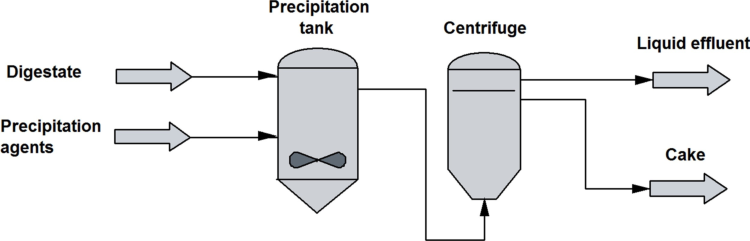
\includegraphics[width=0.8\linewidth, trim={0cm 0cm 0cm 0cm},clip]{gfx/Chapter2/Fig4.pdf} 
	\caption{Scheme for the centrifugation treatment.}
	\label{fig:CentrifScheme}
\end{figure}

Centrifugation process consists of two units, a precipitation tank where CaCO3 and FeCl3 are added, and the centrifuge. These equipment have been modeled using mass balances and removal ratios for the precipitating species. Note that the total solids, carbon, and potassium are assumed to be present in the form of solid compounds, so they will be removed as part of the cake. Moreover, the water content of the centrifuge outlet solids stream is assumed to be 60\% $\left(C_{Wa}^{centrifuge}\right)$ \citep{wakeman2007separation}. Mass balances for the process have been evaluated in Eqs. \ref{eq:Eq51}-\ref{eq:Eq59}:

\begin{align}
	& F_j^{in} = F_{TS}^{in} \cdot \frac{\varphi _{j}}{C_{j}} \label{eq:Eq51} \\
	& {j} \in \left\{ {\text{precipitation agents}} \right\} \nonumber
\end{align}

\begin{align}
	F_j^{in} = F_j^{prec \ tank} = F_j^{centrifuge} = F_j^{cake} \label{eq:Eq52}
\end{align}

\begin{align}
	& F_i^{in} = F_i^{prec \ tank} = F_i^{centrifuge} \label{eq:Eq53} \\
	& {i} \in \left\{ {{\text{P, N}}} \right\} \nonumber
\end{align}

\begin{align}
	F_i^{cake} = F_i^{centrifuge} \cdot {\eta_i} \label{eq:Eq54}
\end{align}

\begin{align}
	F_i^{liquid \ effluent} = F_i^{centrifuge} - F_i^{cake} \label{eq:Eq55}
\end{align}

\begin{align}
	& F_k^{in} = F_k^{prec \ tank} = F_k^{centrifuge} = F_k^{cake} \label{eq:Eq56} \\
	& {k} \in \left\{ \text{TS, C, K} \right\} \nonumber
\end{align}

\begin{align}
	F_{Wa}^{in} = F_{Wa}^{prec \ tank} = F_{Wa}^{centrifuge} \label{eq:Eq57}
\end{align}

\begin{align}
	{F}_{Wa}^{cake} = \left( {F}_{TS}^{cake} + \sum\limits_i {F}_i^{cake} + \sum\limits_j {F}_j^{cake} \right) \cdot \frac{C_{Wa}^{centrifuge}}{1 - C_{Wa}^{centrifuge}} \label{eq:Eq58}
\end{align}

\begin{align}
	{F}_{Wa}^{liquid \ effluent} = F_{Wa}^{centrifuge} - {F}_{Wa}^{cake} \label{eq:Eq59}
\end{align}

where $\varphi _{j}$ is the precipitation agent per total solids mass ratio (0.61 kg CaCO\textsubscript{3}/kg TS and 0.44 kg FeCl\textsubscript{3} /kg TS).

These units have been designed using correlations as a function of the flow processed. For the design of the precipitation tank (volume, diameter, length, thickness, weight, and cost calculations) the equations provided by \citet{almena2016technoeconomic} have been used as before, Eqs. \ref{eq:Eq29}-\ref{eq:Eq37}, considering a hydraulic retention time of 2.5 min \citep{szabo2008significance}.

\begin{align}
	{V}_{Prec tank} \left( \text{m}^{3} \right) = HRT_{Prec \ tank} \cdot \left( \frac{F_{digestate}^{in}}{\rho_{digestate}} + \frac{F_{FeCl_{3}}^{in}}{\rho _{FeCl_{3}}} \right) \label{eq:Eq60}
\end{align}

The volume of CaCO\textsubscript{3} added is assumed negligible compared to the volume of the liquid because it is added as a solid. Thus, the diameter of the tanks is computed using Eqs. \ref{eq:Eq60} and \ref{eq:Eq30} as in the previous unit. The cost of the vessel is given by the weight of the metal, using the correlations provided by \citet{almena2016technoeconomic}, Eqs. \ref{eq:Eq31}-\ref{eq:Eq34}. The power required is computed, as in previous cases, using the rules of thumb in \citet{walas1988chemical}, Eq. \ref{eq:Eq35}, where the value of $\kappa_{agitator}$ agitator is equal to 10 HP per 1000 gal, in accordance with the data collected in the literature \citep{walas1988chemical}. The cost correlation is given by Eq. \ref{eq:Eq36} and updated to 2016 prices. The total cost of the precipitation tank included the vessel and the agitator costs, Eq. \ref{eq:Eq37}.

The centrifuge size is characterized by its diameter. We model it as in the previous technologies using Eqs. \ref{eq:Eq44}-\ref{eq:Eq48}. The operating costs involve fixed, chemicals and labour costs. Fixed costs are estimated using Eq. \ref{eq:Eq61}. The labor cost is estimated in Eq. \ref{eq:Eq13}, where $n_{OP}$ is equal to 1 \citep{vian1975pronostico}. Total operating cost is given by Eq. \ref{eq:Eq14}. The chemicals costs involve the consumption of CaCO\textsubscript{3} and FeCl\textsubscript{3}, and it is estimated using Eq. \ref{eq:Eq62}:

\begin{align}
	{FC}_{centrifugation} \left( \frac{\text{EUR}}{\text{year}} \right) = \left( {Cost_{centrifuge}} + {Cost}_{Prec \ tank} \right) \cdot {f_i} \cdot {f_j} \label{eq:Eq61}
\end{align}

\begin{align}
	& {ChemC}_{centrifugation} \left( \frac{\text{EUR}}{\text{year}} \right) = \label{eq:Eq62} \\
	& \left( F_{CaCO_{3}}^{in} \cdot {Price}_{CaCO_{3}} + F_{FeCl_{3}}^{in} \cdot {Price}_{FeCl_{3}} \right) \cdot 3600 \cdot h \cdot d \nonumber
\end{align}

The cake recovered is the main asset of the process. Its price is estimated as the weighted sum of each nutrient, Eq. \ref{eq:Eq15}, \citep{hernandez2017bio}. Finally, the benefits or losses of operating this system are calculated as the difference between the revenue obtained from the cake and the operating costs of the facility, Eq. \ref{eq:Eq16}.

\subsubsection{Struvite production}
P and N can be recovered from digestate through the formation of struvite, which is a phosphate mineral with a chemical formula of MgNH\textsubscript{4}PO\textsubscript{4} ·6H\textsubscript{2}O. The advantage of this technology is that struvite is a solid with a high nutrients density, it is easy to transport, and it can be used as slow-release fertilizer without any post-processing \citep{doyle2002struvite}. The removal of nutrients via struvite production follows the reaction below, requiring the addition of MgCl\textsubscript{2}, resulting in the production of struvite crystals that can be recovered as solid:

\begin{align}
	\text{Mg}^{2+} + \text{NH}_4^{+}  + \text{H}_{\text{n}}\text{PO}_4^{3-n} + 6\text{H}_{2}\text{O} \leftrightarrow \text{MgNH}_{4}\text{PO}_{4} \cdot 6\text{H}_{2}\text{O} + \text{nH}^{+} \label{eq:Eq63}
\end{align}

Due to the presence of potassium in the digestate, together with struvite, another product called potassium struvite or K-Struvite, is also produced. In this case the ammonia cation is substituted by the potassium cation \citep{wilsenach2007phosphate}.

\begin{align}
	\text{K}^{+} + \text{Mg}^{2+} + \text{H}_{\text{n}}\text{PO}_4^{3-n} + 6\text{H}_{2}\text{O} \leftrightarrow \text{KMgPO}_{4}\cdot 6\text{H}_{2}\text{O} + \text{nH}^{+} \label{eq:Eq64}
\end{align}

Since the formation of struvite is favored over the formation of K-Struvite, it is considered that only 15\% of the potassium contained in the digestate will react to form K-Struvite \citep{zeng2006nutrient}. The mass balance for the reactors is given by the stoichiometry of the reactions above.

Two different types of reactors can be used to obtain struvite, either a stirred tank (CSTR) or a fluidized bed reactor (FBR). Figs. \ref{fig:FBRScheme} and \ref{fig:CSTRScheme} provide detailed flowsheets of each case. In case of the FBR, struvite is recovered from the bottoms and the liquid must be processed in a hydrocyclone to avoid discharging fines. In the case of CSTR tanks, we need to use a centrifuge to recover the struvite. We can help the crystal growth by seeding \citep{doyle2002struvite, kumashiro2001pilot}. Due to the substantial increase in the struvite formation yield, we consider the addition of struvite seeds in both cases. The reaction takes place at about 27 \textdegree C, with the addition of MgCl\textsubscript{2} at a concentration of 57.5 mg/dm\textsuperscript{3} \citep{zhang2014phosphate}. A Mg:P molar ratio of 2 \citep{bhuiyan2008phosphorus} is used.

\begin{figure}[h!]
	\centering
	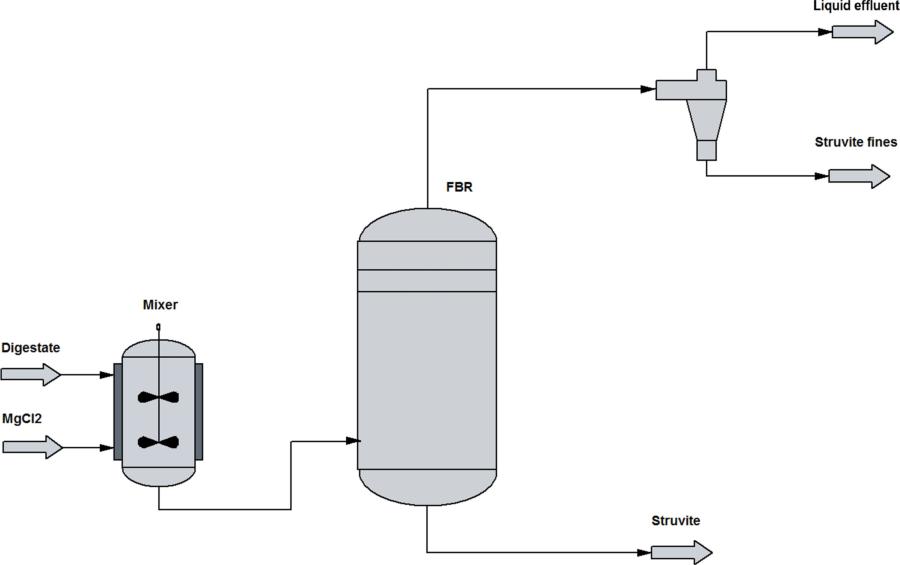
\includegraphics[width=0.8\linewidth, trim={0cm 0cm 0cm 0cm},clip]{gfx/Chapter2/Fig5.pdf} 
	\caption{Scheme for the FBR system.}
	\label{fig:FBRScheme}
\end{figure}

\begin{figure}[h!]
	\centering
	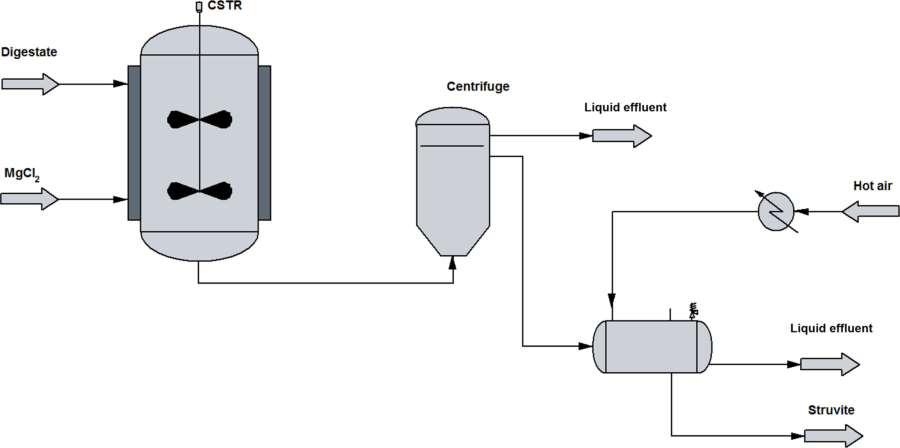
\includegraphics[width=0.8\linewidth, trim={0cm 0cm 0cm 0cm},clip]{gfx/Chapter2/Fig6.pdf} 
	\caption{Scheme for the CSTR based struvite production system.}
	\label{fig:CSTRScheme}
\end{figure}

The FBR system is composed of three elements: a mixer tank, a FBR rector, and a hydrocyclone. The system operation consists of a digestate flow which is mixed with a stream of MgCl\textsubscript{2} in the mixing tank. The addition of MgCl\textsubscript{2} helps precipitate the struvite by increasing the concentration of the species inside the reactor. As the concentration of NH\textsuperscript{4+} is high due to the pH, and the inorganic N and P are the elements we want to recover, the only element which is necessary to be added is Mg in form of MgCl\textsubscript{2}.

In the tank there is a suspension of struvite seeds with a size of 0.8 mm which promote the precipitation of struvite. The solid struvite is evacuated from the reactor at the bottom and its moisture is low enough to avoid the use of a dryer. The other stream which leaves the reactor contains liquid water in a high proportion with the excess of Mg, the total solids from the digestate, and low amounts of nutrients and other components. This stream is introduced in a hydrocyclone to recover fines of struvite which can be removed by this stream. 100\% of fines removal is assumed but no fines production is considered in the model.

To estimate the cost of this system we evaluate the effect of the following variables, whose operating values are shown between parenthesis:

\begin{itemize}
	\item Digestate input mass and volume flow (between 1 and 100 kg/s)
	\item Recovered struvite humidity (5\% in mass)
	\item Amount of phosphorus recovered (90\%)
	\item Mg:P molar ratio with a value of 2
\end{itemize}

In an FBR there are some variables which influence in the design and hence the cost. The variables considered in this work are showed below with the typical values used in the present study between parenthesis:

\begin{itemize}
	\item $d_p$: bed particle diameter, assumed to be 0.8 mm \citep{jordaan2011development}
	\item Sphericity: 0.6 is a standard sphericity for particles used in fluidized bed reactors \citep{Fogler2005Elements}
\end{itemize}

Furthermore, the reaction kinetics and equilibrium are considered to estimate the residence time in the reactor. A first order kinetics, developed by \citet{nelson2003struvite}, has been used, Eqs. \ref{eq:Eq65} and \ref{eq:Eq66}. The kinetic constant is $3.42 \cdot 10^{-3}$ s \textsuperscript{-1} for a pH of 9.

\begin{align}
	\frac{{-dC}}{{dt}} = k \left({C - {C_{eq}}} \right) \label{eq:Eq65}
\end{align}

\begin{align}
	\ln \left( {C - {C_{eq}}} \right) =  - kt + \ln \left( {{C_0} - {C_{eq}}} \right) \label{eq:Eq66}
\end{align}

Struvite formation is an equilibrium reaction. We use the equilibrium ion activity product $\left(IAP_{eq}\right)$ value of $7.08 \cdot 10^{-14}$ \citep{nelson2003struvite} to calculate the equilibrium concentrations in the kinetic model, Eq. \ref{eq:Eq67}. We assumed that the values of ions concentration are equal to ions activity.

\begin{align}
	IAP_{eq} = \left( {Mg^{2+}} \right)\left( NH_4^{+} \right)\left( {PO_4^{3-}} \right) = 7.08 \cdot {10^{ - 14}}  \label{eq:Eq67}
\end{align}

Minimum fluidization velocity is calculated in the first step by considering that the fluid stream is a liquid \citep{mangin2004fluid}. This consideration is motivated because the liquid digestate works as fluidization agent \citep{le2006understanding}. The digestate density is 950 kg/m\textsuperscript{3} \citep{rigby2011new}. The expression used to calculate $u_{mf}$ through Reynolds and Archimedes numbers is given by Eq. \ref{eq:Eq68}, \citep{tisa2014basic}.

\begin{align}
	{u_{mf}} = \frac{Re_{l \ mf} \cdot {\mu_{digestate}}}{\rho_{digestate} - {d_p}} \label{eq:Eq68}
\end{align}

Eq. \ref{eq:Eq68} parameters are determined by Eqs. \ref{eq:Eq69} and \ref{eq:Eq70}.

\begin{align}
	Re_{l \ mf} = \sqrt {33.72 + 0.0404Ar_{l}{\left( {1 - {\alpha_{mf}}} \right)^3}} - 33.7 \label{eq:Eq69}
\end{align}

\begin{align}
	Ar_{l} = \rho_{digestate} \left( {\rho_{struvite} - {\rho _{digestate}}} \right) g \frac{d_p^3}{\mu_{digestate}^2} \label{eq:Eq70}
\end{align}

If the flow has no gas phase, $\alpha_{mf}$ is equal to zero. The terminal velocity is computed using Eq. \ref{eq:Eq71} \citep{tisa2014basic}.

\begin{align}
	{u_t} = \left( \frac{1.78 \cdot {10}^{ - 2} \cdot {\eta ^2}}{\rho_{digestate} \cdot \mu _{digestate}} \right)^{1/3} {d_p} \label{eq:Eq71}
\end{align}

where the parameter $\eta$ is given by Eq. \ref{eq:Eq72}:

\begin{align}
	\eta  = g\left( {\rho _{struvite} - {\rho _{digestate}}} \right) \label{eq:Eq72}
\end{align}

Finally, the fluid velocity $u_0$ must be between $u_{mf}$ and $u_t$. A superficial velocity equal to five times the minimum fluidization velocity is selected \citep{tejero2004optimization}, Eqs. \ref{eq:Eq73} and \ref{eq:Eq74}.

\begin{align}
	{u_{mf}} < {u_0} < {u_t} \label{eq:Eq73}
\end{align}

\begin{align}
	{u_0} = 5 \cdot {u_{mf}} \label{eq:Eq74}
\end{align}

Once the superficial velocity is computed, the area and diameter can be calculated from the mass flow Eqs. \ref{eq:Eq75} and \ref{eq:Eq76}.
\begin{align}
	{A_{FBR}} = \frac{F_{digestate}^{in}}{u_0} \label{eq:Eq75}
\end{align}

\begin{align}
	{D_{FBR}} = \sqrt {\frac{4{A_{FBR}}}{\pi}} \label{eq:Eq76}
\end{align}

The length of the bed is determined by the residence time through the kinetics and the equilibrium ion activity product presented above. Consequently, the magnesium and ammonium concentrations can be calculated from the digestate mass balance and the external magnesium added. Using the $IAP_{eq}$ value, the phosphate concentration in equilibrium at the operational conditions can be determined. This equilibrium value will be used in kinetics, Eq. \ref{eq:Eq77}.

\begin{align}
	t = \frac{\ln \left( {C_0} - {C_{eq}} \right) - \ln \left( C - {C_{eq}} \right)}{k} \label{eq:Eq77}
\end{align}

Thus, the bed length is computed as per Eq. \ref{eq:Eq78}. Typically, the length of the reactor must be 15\% larger than the bed, Eq. \ref{eq:Eq79}.

\begin{align}
	L_{bed} = u_0 \cdot t \label{eq:Eq78}
\end{align}

\begin{align}
	L_{FBR} = 1.15 \cdot L_{bed} \label{eq:Eq79}
\end{align}

The estimation of the rector cost is carried out assuming that it is a vessel as presented in the processes above, Eqs. \ref{eq:Eq30}-\ref{eq:Eq34} \citep{almena2016technoeconomic}. The cost of the mixer tank is also estimated as that of a vessel, using Eqs. \ref{eq:Eq29}-\ref{eq:Eq34}, with a volume given by that to provide a hydraulic retention time of 150 s \citep{szabo2008significance}. The impeller is also designed using the same procedure as before, Eqs. \ref{eq:Eq35} and \ref{eq:Eq36} \citep{walas1988chemical}.

Finally, to estimate the cost of the hydrocyclone, a surrogate model using data from Matche website has been developed \citep{Matche} (\url{www.matche.com}). There is a maximum diameter, therefore, if a unit larger than the standard is required, we actually need to duplicate the equipment, Eq. \ref{eq:Eq81}. To estimate the diameter, we considered that there is a linear relationship between the diameter and the flow based on rules of thumb in design literature. A typical unit size of a 20 in diameter hydrocyclone can process 1,000 US gallons per min, Eq. \ref{eq:Eq80} \citep{walas1988chemical}.

\begin{align}
	{D}_{hydrocyclone}\left( {\text{in}} \right) = F_{digestate}^{in} \left( \frac{\text{US gallon}}{\text{min}} \right) \cdot \frac{20}{1000} \label{eq:Eq80}
\end{align}

\begin{align}
	{n}_{hydrocyclone} \ge \frac{D^{hydrocyclone}}{D_{max}^{hydrocyclone}} \label{eq:Eq81}
\end{align}

where ${n}_{hydrocyclone}$ is an integer. The maximum diameter for a hydrocyclone, $D_{max}^{hydrocyclone}$,  is 30 inch based on standard sizes (\url{www.matche.com}).  Thus, the design diameter is the lower diameter between $D^{hydrocyclone}$ and $D_{max}^{hydrocyclone}$, Eq. \ref{eq:Eq82}.

\begin{align}
	D_{design}^{hydrocyclone} = \min (D_{total}^{hydrocyclone}, \ D_{max}^{hydrocyclone}) \label{eq:Eq82}
\end{align}

The estimation of the cost for the fines recovery equipment is computed using Eq. \ref{eq:Eq83} and updated as explained above.

\begin{align}
	& Cost_{hydrocyclone} \left( \text{USD}_{2014} \right) = \label{eq:Eq83} \\
	& {n}_{hydrocyclone} \cdot \left( {2953.2} \cdot D_{design}^{hydrocyclone} - 34,131 \right) \nonumber
\end{align}

The CSTR process consists of four elements: the CSTR reactor, a centrifuge, and a dryer with its corresponding heat exchanger. As the residence time in the CSTR is large enough, it is not necessary to use a mixing tank and MgCl\textsubscript{2} is added directly in the reactor. Thus, struvite is formed in one step in the CSTR. Since the digestate already contains NH\textsubscript{4}\textsuperscript{+} and P, we need to add MgCl\textsubscript{2}. As a result, struvite precipitates, and it is recovered from the bottoms of the reactor and dried in a two step process. The first step consists of a centrifuge that recovers struvite with 5\% (on weight basis) water \citep{baasal1989preliminary}. Next, a drum dryer is implemented to remove the residual moisture to reach commercial standards and reduce transportation costs. Fig. \ref{fig:CSTRScheme} shows the details of the flowsheet. 

The design of the units involved in this process and their cost estimation is based on the following variables:

\begin{itemize}
	\item Digestate input mass and volume flow (between 1 and 100 kg/s)
	\item Recovered struvite humidity (5\% in mass)
	\item Amount of phosphorus recovered (90\%)
	\item Mg:P molar ratio with a value of 2
\end{itemize}

The CSTR is assumed to be a stirred vessel; consequently, it is designed as in the previous cases, Eqs. \ref{eq:Eq29}-\ref{eq:Eq37}, with a residence of 471.05 s. The residence time is calculated from mass balances and the kinetics described in the FBR process, Eqs. \ref{eq:Eq65} and \ref{eq:Eq66}.

The centrifuge size is characterized by its diameter. Both, the size and cost are computed using the data in \citet{green2008perry}. We assume a pusher type for the centrifuge with a maximum diameter of 1250 mm as before, Eqs. \ref{eq:Eq44}-\ref{eq:Eq48}.

The cost estimation for the dryer relies on the amount of water to evaporate, and the evaporation capacity. The evaporation capacity $\left(e_{capacity}\right)$ is reported in the literature to be equal to 0.01897 (kg/(s $\cdot$ m\text{2})) \citep{walas1988chemical}. Consequently, the dryer cost is computed using a correlation provided by \citet{martin2011energy}, Eq. \ref{eq:Eq84}, updating the cost to current prices using the Chemical Engineering Index.

\begin{align}
	Cost_{dryer}\left( \text{USD}_ {2007} \right) = 1.15 \cdot \left( {6477.1 \cdot \frac{F_{water}^{in}}{e_{capacity}} + 102394} \right) \label{eq:Eq84}
\end{align}

The operating cost of the CSTR and the FBR based processes is computed considering three items, fixed, chemicals and labor, and assuming that utilities account for 20\% of the operating costs. The correlations for computing each of them are taken from \citet{vian1975pronostico} and \citet{sinnott1999chemical}, Eq. \ref{eq:Eq13} for labour and Eq. \ref{eq:Eq14} for total operating cost. Fixed cost for struvite processes is calculated using Eq. \ref{eq:Eq85}. We assume that the seeds required for the FBR process are internally produced in the startup of the facility.

\begin{align}
	FC_{struvite} \left( \frac{\text{EUR}}{\text{year}} \right) = \left( \sum {Cost_{equipment}} \right) \cdot {f_i}\cdot{f_j} \label{eq:Eq85}
\end{align}

The revenue obtained from the struvite is determined assuming a selling price of 0.763D EUR/kg, Eq. \ref{eq:Eq86}, \citep{molinos2011economic}.

\begin{align}
	Cost_{struvite} \left( \frac{\text{EUR}}{\text{year}} \right) = \left( F_{struvite}^{recovered}\cdot{Price}_{struvite} \right) \cdot 3600\cdot h \cdot d \label{eq:Eq86}
\end{align}

Finally, the benefits or losses for CSTR and FBR are calculated as the difference between the credit obtained from the struvite and the operating costs of the facility, Eq. \ref{eq:Eq16}.


\subsection{Solution procedure} \label{section:SolutionProcedure}
The detailed models for each of the alternatives such as the five filter media or the number of different coagulants result in a large and complex MINLP when cost estimation is involved. We use a two-stage procedure to select the best technology. In the first stage we develop MINLP subproblems to select the appropriate filter media or coagulant. Next, using the detailed models for the best option, surrogate cost models are developed for the five alternative technologies used to process the digestate. However, there are still binary decisions to account for the cost of the active alternative in the superstructure. Thus, the surrogate models are in the form of linear equations. For instance, the surrogate model for the filter to be implemented in the superstructure is given by a linear function as given by Eq. \ref{eq:Eq87}.

\begin{align}
	&{Operating \ cost} \left( \frac{\text{EUR}}{\text{year}} \right) =  \label{eq:Eq87} \\
	& 20,521 \cdot F_{design} \left( \frac{\text{ft}{^3}}{\text{min}} \right) { -33,488} \cdot {a}_{Filter} \nonumber
\end{align}

We avoid the use of binary variables within the formulation (due to highly non linear model of the entire superstructure) by using smooth approximations. We define $a_{Filter}$ as a parameter that takes a value of 0 when $F_{design}^{Filter}$ is 0 and 1 if $F_{design}^{Filter}$ is not equal to 0. The smooth approximation for $a_{Filter}$ is defined as follows, Eq. \ref{eq:Eq88}:

\begin{align}
	a_{Filter} = \frac{1}{1 + {e^{\left( -{F_{design}} + {0.049} \right) \cdot 361}}} \label{eq:Eq88}
\end{align}

Metal slag is selected as the best filter for the filtration process. For the case of the coagulants, the solution of the subproblem, Eqs. \ref{eq:Eq17}-\ref{eq:Eq50} selects the use of AlCl\textsuperscript{3}. As in the previous case, a surrogate model is developed to be included in the superstructure so that we avoid including binary variables and allow for zero operating costs in case this technology is not selected, Eq. \ref{eq:Eq89}.

\begin{align}
	& {Operating \ cost} \left( \frac{\text{EUR}}{\text{year}} \right) = \label{eq:Eq89} \\
	& 1,019,589.91 \cdot F_{digestate}^{in} \left( \frac{\text{kg}}{\text{s}} \right) -368,838.56 \cdot {a}_{Coag} \nonumber
\end{align}

where the smooth approximation for the term ${a}_{Coag}$ is given by Eq. \ref{eq:Eq90}.

\begin{align}
	{a}_{Coag} = \frac{1}{1 + e^{\left( -F_{digestate}^{in} + 0.068 \right) \cdot 863}} \label{eq:Eq90}
\end{align}

Similar to previous cases we develop a surrogate model to estimate the operating cost for the centrifugation as a function of the flowrate of digestate, Eq. \ref{eq:Eq91}:

\begin{align}
	& {Operating \ cost} \left( \frac{\text{EUR}}{\text{year}} \right) = \label{eq:Eq91} \\
	& 458,498.29 \cdot F_{digestate}^{in} +  24,924.67 \cdot {a}_{Centrifugation} \nonumber
\end{align}

As before, ${a}_{Centrifugation}$ is approximated as follows, Eq. \ref{eq:Eq92}:

\begin{align}
	{a}_{Centrifugation} = \frac{1}{1 + e^{\left( { - F_{digestate}^{in} + 0.068} \right) \cdot 863}} \label{eq:Eq92}
\end{align}

Finally, to include the operating costs for the production of struvite, we again develop surrogate models for the FBR, Eq. \ref{eq:Eq93} and for the CSRT Eq. \ref{eq:Eq95}, where a smooth approximation is proposed for the fixed term, $a_{FBR}$ and $a_{CSTR}$ respectively, Eqs. \ref{eq:Eq94} and \ref{eq:Eq96}.

\begin{align}
	{Operating \ Cost}_{FBR} \left( \frac{\text{EUR}}{\text{year}} \right) = 245,008 \cdot F_{digestate}^{in} +  1 \cdot {10^6} \cdot {a}_{FBR} \label{eq:Eq93}
\end{align}

\begin{align}
	{a}_{FBR} = \frac{1}{1 + {e^{\left( { - F_{digestate}^{in} + 0.06785} \right) \cdot 862.9679}}} \label{eq:Eq94}
\end{align}

\begin{align}
	&{Operating \ Cost}_{CSTR} \left( \frac{\text{EUR}}{\text{year}} \right) = \label{eq:Eq95} \\
	& 277,051 \cdot F_{digestate}^{in} +  1 \cdot {10^6} \cdot {a}_{CSTR} \nonumber
\end{align}

\begin{align}
	{a}_{CSTR} = \frac{1}{1 + {e^{\left( { - F_{digestate}^{in} + 0.06785} \right) \cdot 862.9679}}} \label{eq:Eq96}
\end{align}

The benefits/losses in the superstructure for any of the technologies to process the digestate is computed as the difference between the revenue obtained from the nutrients and generated power, and the operating costs of the facility.

Finally, the whole superstructure is built (see Fig. \ref{fig:Flowsheet}). This superstructure contains models of the fermenter, biogas purification, gas cycle, steam cycle, and digestate treatment processes. The aim of this superstructure is to determine the optimal operating conditions and to select the best digestate treatment technology. Thus, digestate treatment processes have been implemented in the superstructure through detailed mass balances including the solution to the kinetics of the fluidized bed reactors as well as the surrogate models developed in the previous stage to estimate the operating costs. It should be noted that in filtration, centrifugation, and coagulation processes we have included a benefits penalty, $F^{recovered}_{total}$, due to the fact that the product recovered is a mixture of nutrients and organic matter with a nutrients concentration lower than struvite. This penalty represents the concentration of nutrients in the recovered product given by the ratio between the nutrients recovered and the total recovered mass flow, Eq. \ref{eq:Eq97}.

\begin{align}
	& {Price} \left( \frac{\text{EUR}}{\text{year}} \right) = \label{eq:Eq97} \\ 
	& \left( {F_P^{recovered}\cdot{Price}_P} + F_N^{recovered} \cdot {Price}_N + F_{K}^{recovered} \cdot {Price}_K \right) \nonumber\\
	& \cdot \frac{1}{F_{total}^{recovered}} \cdot 3600 \cdot h\cdot d \nonumber
\end{align}

The total energy obtained in the system to be optimized is the sum of the one generated at the three sections of the turbine, high, medium and low pressure and that of the gas turbine. We use part of the energy produced to power the compressors used across the facility. The economic benefits or losses of each digestate treatment process are added to the energy benefits.

\begin{align}
	&Z = \Bigg[ \left( \sum\limits_{i \in Turbines} {W}_{ {Turbine} }  + W_{Gas \ Turbine} - \sum\limits_{j \in Compressors} W_{Compressors}  \right) \label{eq:Eq98} \\ 
	& \cdot 3600\cdot h \cdot d \cdot {C_{Electricity}} \Bigg]+ Benefits_{Filtration} + {Benefits}_{Centrifugation} + \nonumber \\
	& {Benefits}_{Coagulation} + {Benefits}_{FBR} + {Benefits}_{CSTR} \nonumber
\end{align}

Eq. \ref{eq:Eq98} is the objective function that we maximize to determine the optimal operational conditions and to select the best digestate treatment process subject to the following constraints:

\begin{itemize}
	\item Bioreactor and biogas composition model. Described in Section \ref{section:BiogasProduction}
	\item Digestate processing. Described in Section \ref{section:DigestateConditioning}
	\item Biogas purification. Described in Section \ref{section:BiogasPurification}
	\item Brayton cycle. Described in Section \ref{section:BraytonCycle}
	\item Rankine cycle. Described in Section \ref{section:RankineCycle}
\end{itemize}

The main decision variables are related to the selection of the digestate processing technology, among filtration, centrifugation, coagulation and struvite production using CSTR or FBR. The decision variables are also associated with the selection of the type of filter and the coagulation agent. Furthermore, the biogas usage to produce steam requires the operating pressures and temperatures at the gas turbine, and the steam turbine as well as the extraction form the steam turbine to reheat the condensate before regenerating steam using the flue gas from the gas turbine. The superstructure consists of an NLP of approximately 4,000 equations and 5,000 variables solved using a multistart procedure with CONOPT 3.0 as the preferred solver. The computational time is around 60 min, although it varies for each problem as a consequence of the different data used in each case.

\begin{table}[h!]
	\centering
	\caption{Operating data of the optimal configuration for each raw material.}
	\label{table:Table4}
	\resizebox{0.75\columnwidth}{!}{
	\begin{tabular}{@{}lllll@{}}
		\toprule
		&               & T (\textdegree C)      & P (bar)    & Extractions  \\ \midrule
		Cattle  & Bioreactor    & 55          & 1          & –            \\
		& Gas turbine   & 2430 (in)   & 8.2 (in)   & –            \\
		&               & 1205 (out)  & 1 (out)    &              \\
		& Steam turbine & 1000 (T1)   & 125 (P1 )  & 6.7\% to HX7 \\
		&               & 568 (T2 )   & 11 (P2 )   &              \\
		&               & 442 (T3 )   & 5 (P3 )    &              \\
		&               & 41.8 (T4 )  & 0.08 (P4 ) &              \\
		& FBR           & 25          & 1          & –            \\
		Pig     & Bioreactor    & 55          & 1          & –            \\
		& Gas turbine   & 2430 (in)   & 8.2 (in)   & –            \\
		&               & 1205 (out)  & 1 (out)    &              \\
		& Steam turbine & 1000 (T1)   & 125 (P1 )  & 6.7\% to HX7 \\
		&               & 568 (T2 )   & 11 (P2 )   &              \\
		&               & 442 (T3 )   & 5 (P3 )    &              \\
		&               & 41.8 (T4 )  & 0.08 (P4 ) &              \\
		& FBR           & 25          & 1          & –            \\
		Poultry & Bioreactor    & 55          & 1          & –            \\
		& Gas turbine   & 2430 (in)   & 8.2 (in)   & –            \\
		&               & 1205 (out)  & 1 (out)    &              \\
		& Steam turbine & 1000 (T1)   & 125 (P1 )  & 6.7\% to HX7 \\
		&               & 568 (T2 )   & 11 (P2 )   &              \\
		&               & 442 (T3 )   & 5 (P3 )    &              \\
		&               & 41.8 (T4 )  & 0.08 (P4 ) &              \\
		& FBR           & 25          & 1          & –            \\
		Sheep   & Bioreactor    & 55          & 1          & –            \\
		& Gas turbine   & 2337 (in)   & 15.6 (in)  & –            \\
		&               & 896 (out)   & 1 (out)    &              \\
		& Steam turbine & 769.6 (T1 ) & 95 (P1 )   & 2.9\% to HX7 \\
		&               & 439.1 (T2 ) & 11 (P2 )   &              \\
		&               & 329.6 (T3 ) & 5 (P3 )    &              \\
		&               & 73.0 (T4 )  & 0.35 (P4 ) &              \\
		& FBR           & 25          & 1          & –            \\ \bottomrule
	\end{tabular}
	}
\end{table}

\section{Results} \label{section:Results}
Following the optimization procedure presented in Section \ref{section:SolutionProcedure} we first decide on the filter media and the coagulant chemical. We solve MINLP subproblems leading to the selection of the filter media and the coagulant agent. We use the metal slag as the filter media and the AlCl\textsubscript{3} as the coagulant for all raw materials. Next, we developed surrogate models for the five technologies included in the superstructure and solve a reformulated NLP including smooth approximations for the cost functions of the digestate treatment so as to maximize the power produced and the treatment section. The plant size is assumed to be that which processes 10 kg/s of manure based on the typical amount of manure produced in cattle farms \citep{LeonMsc}. Four manures have been evaluated on the plant: cattle, pig, poultry and sheep, with the aim of determining, for each one, the power generated the composition of the biogas produced, the optimal digestate treatment technology to recover its nutrients and the biogas-manure and digestate-manure ratios. Section \ref{section:Balanaces} summarizes the main operating conditions of the major units in the process and the selection of digestate processing technology. Section \ref{section:EconomicEvaluation} presents the detail economic evaluation of the four optimal processes, one per manure type. Finally, in Section \ref{section:Effect} an analysis of the effect of the manure composition on the power, operating conditions and digestate treatment is performed.


\subsection{Mass and energy balances} \label{section:Balanaces}
Table \ref{table:Table4} shows the main operating conditions of major units for the four different manure types. Cattle, pig, and poultry show similar values among them and to previous work \citep{Leon}. The gas in the gas turbine reaches a temperature of 2400 \textdegree C and a pressure of 8.2 bar before expansion for cattle, pig and poultry manure. However, sheep manure shows different values. While the temperature is similar, the pressure is 15.6 bar, almost twice the value found for the rest of the raw materials. Furthermore the flue gas exits the turbine 300 \textdegree C below that when the rest of the manure types are used. Furthermore while the high pressure of the steam turbine is 125 bar for cattle, pig, and poultry manure, in case of sheep manure the steam turbine operates at 95 bar at the high pressure section of the turbine. This is related to the lower gas temperature from the gas turbine since the overheated steam needs to be produced using that stream. Intermediate and low pressures are the same in the steam turbine using any of the manure types, but the exhaust pressure of the steam is higher in case of sheep manure. Table \ref{table:Table5} shows the products obtained from the various manure types, power, biogas, and digestate. Poultry is the waste that is more efficient towards power production due to its higher concentration. In all cases an FBR reactor for the production of struvite is the selected technology to recover N and P. In the table we also see the effect of the fact that cattle and pig manure are mostly liquids, since most of the product is digestate, almost 98\%, while the use of poultry or sheep manure reduces the production of digestate to 75\% and 88\% respectively, increasing the production of biogas and power. Finally in Table \ref{table:Table6} the biogas composition for each manure considered are presented. The main purpose of the facility is the production of power. However, the biogas composition is typically within a range of values per component that have been imposed as bounds. As a result of maximizing the electricity production for all studied cases, the same biogas composition is obtained, 67.5\% molar in CH\textsubscript{4} and the rest is mostly CO\textsubscript{2}.

\begin{table}[h!]
	\centering
	\caption{Process optimization results for considered manures.}
	\label{table:Table5}
			\resizebox{0.95\columnwidth}{!}{
		\begin{tabular}{@{}ccccccc@{}}
			\toprule
			Manure  & \begin{tabular}[c]{@{}c@{}}Power\\ (kW)\end{tabular} & \begin{tabular}[c]{@{}c@{}}Comp. biogas\\ (CH\textsubscript{4}/CO\textsubscript{2}\\ratio)\end{tabular} & \begin{tabular}[c]{@{}c@{}}Digestate \\treatment \\ technology\end{tabular} & \begin{tabular}[c]{@{}c@{}}Product\\ recovered\end{tabular} & \begin{tabular}[c]{@{}c@{}}Biogas/\\manure\\ ratio\end{tabular} & \begin{tabular}[c]{@{}c@{}}Digestate/\\manure\\ ratio\end{tabular} \\ \midrule
			Cattle  & 2,612                                                & 0.816                                                                  & FBR struvite                                                              & Struvite                                                    & 0.0208                                                        & 0.9794                                                           \\
			Pig     & 2,612                                                & 0.816                                                                  & FBR struvite                                                              & Struvite                                                    & 0.0208                                                        & 0.9794                                                           \\
			Poultry & 31,349                                               & 0.818                                                                  & FBR struvite                                                              & Struvite                                                    & 0.2499                                                        & 0.7526                                                           \\
			Sheep   & 14,106                                               & 0.818                           \ref{table:Table4}                                       & FBR struvite                                                              & Struvite                                                    & 0.1217                                                        & 0.8795                                                           \\ \bottomrule
		\end{tabular}
				}
\end{table}

\begin{table}[h!]
	\centering
	\caption{Process optimization results for considered manures.}
	\label{table:Table6}
	\resizebox{0.9\columnwidth}{!}{
		\begin{tabular}{@{}cccccc@{}}
			\toprule
			Manure  & CH\textsubscript{4} (\%wt) & CO\textsubscript{2} (\%wt) & Water (\%wt) & O\textsubscript{2} (\%wt) & N\textsubscript{2} (\%wt) \\ \midrule
			Cattle  & 0.385      & 0.470     \ref{table:Table4} & 0.120        & 0.006     & 0.020     \\
			Pig     & 0.385      & 0.470      & 0.120        & 0.006     & 0.020     \\
			Poultry & 0.385      & 0.470      & 0.120        & 0.006     & 0.020     \\
			Sheep   & 0.385      & 0.470      & 0.120        & 0.006     & 0.020     \\ \bottomrule
		\end{tabular}
	}
\end{table}

\subsection{Economic evaluation} \label{section:EconomicEvaluation}
This section is divided into the estimation of the investment cost, using a factorial method based on the cost of the units, and the estimation of the electricity production cost.

\subsubsection{Investment cost}
We use the factorial method to estimate the investment cost for this facility. This is based on the estimation of the equipment cost and several coefficients to account for pipes, installation, etc. (Sinnott and Towler, 2009). The cost for the different units has been estimated based on \citet{Matche} website (\url{www.matche.com}), \citet{towler2009chemical} and \citet{peters2003plant}, updating the cost of the units when required. We assume a plant that processes fluids and solids. Due to the different composition of each manure the specific production of biogas for each one is different, being larger for poultry and sheep than for cattle and pig. The reason for that could be that sheep and poultry manures have less water content while the water content in cattle and pig reaches 98\% (\url{http://adlib.everysite.co.uk}). For cost estimation proposes the digester maximum size considered is 6,000 m\textsuperscript{3} per unit, since the larger units could face mixing and homogenization problems \citep{rohstoffe2010guia}. This result for the facility investment cost will be different for each raw material. Fig. \ref{fig:CostDist} shows the equipment cost distribution where digester and gas turbine are the most important contributions:

\begin{itemize}
	\item \textbf{Cattle manure:} a plant that processes 10 kg/s of this type of manure requires an investment of 69.1 M EUR, of which 14.9 M EUR represents the equipment cost. The larger cost is assumed by the digester units, with a 75\% of the total units cost, followed by the heat exchanger network with a contribution of 12\% while both turbines add up to 12\%.
	
	\item \textbf{Pig manure:} a facility to process 10 kg/s of this manure requires in an investment of 69.5 M EUR, with a cost of 14.9 M EUR in equipment. Since the digestate-manure and biogas-manure ratios between cattle and pig manure are very similar, the investment	costs are analogous among them. The unit cost distribution is similar to the cattle manure case.
	
	\item \textbf{Poultry manure:} The investment for a plant that processes 10 kg/s of this manure is 208.0 M EUR. The units investment adds up to 44.7 M EUR. In this case the units cost distribution is more homogeneous among different items: 60\% to digester units, 20\% to gas turbine, 10\% to heat exchanger network and 9\% to steam turbine. It should be noted that, as poultry manure has a	high content of dry matter (around 60\% on a weight basis), it is necessary to add additional water to decrease the dry matter content to reach 25\% with the aim of avoid mixing problems in the digester due to an excessive solids concentration inside.
	
	\item \textbf{Sheep manure:} The facility to treat 10 kg/s of this manure requires an investment of 105.0 M EUR, where 22.5 M EUR represents the equipment cost. For this plant the main units cost distribution is as follows: 50\% for the digester, 25\% for gas turbine, 17\% for heat exchanger network and 7\% for steam turbine.
\end{itemize}

\begin{figure}[h]
	\centering
	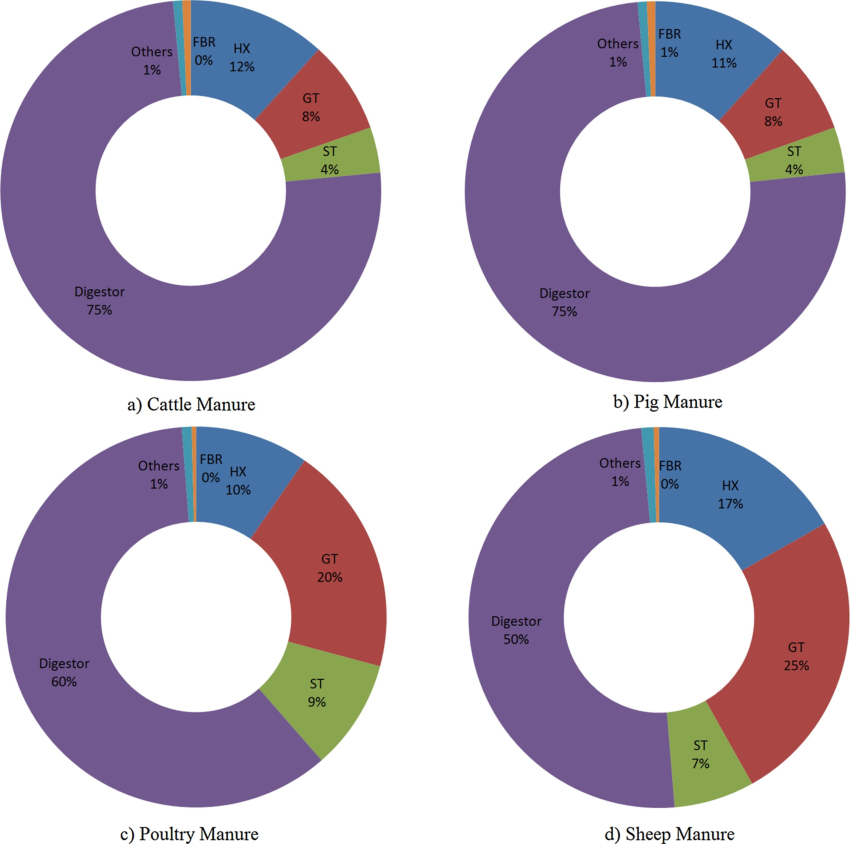
\includegraphics[width=0.8\linewidth, trim={0cm 0cm 0cm 0cm},clip]{gfx/Chapter2/Fig7.pdf} 
	\caption{Units cost distributions for cattle, pig, poultry and sheep manure treatment (ST: steam turbine, GT: gas turbine, HX: heat exchangers, FBR: fluidized bed reactor).}
	\label{fig:CostDist}
\end{figure}

It is clear that the digester shows the largest share in the investment cost and therefore the concentration of the manure highly determines the cost of the facility. \citet{lantz2012economic} presented the investment cost of a facility for heat and power production as a function of its scale. Actually, our plant does not produce steam as a final product but only power. Thus, it is interesting to see that the raw material determines the investment per kW from the 4,000 EUR/kW in case of poultry manure or the 7,500 EUR/kW in case of sheep manure, to the more than 25,000 EUR/kW in case of pig and cattle.

\subsubsection{Production cost}
To calculate the production cost, 20 years of plant life is considered, with a capacity factor of 98\%. Apart from the equipment amortization, other items are also taken into account such as salaries, administrative fees, chemicals cost, maintenance cost, utilities and contingency costs. Thus, apart from the annualized equipment cost, 1.5 M EUR are spent in salaries, 0.25 M EUR in Administration, 2 M EUR in Maintenance, 0.25 M EUR in other expenses \citep{Leon} while chemicals are computed as described in Section \ref{section:ProcessDescription}. The cost of utilities adds up to 0.08 M EUR, accounting for the cooling water and the steam needed to maintain the operation of the digester and to condition the digestate for its use as a fertilizer. Finally, we assume that the livestock manure is for free. Fig. \ref{fig:OpCost} shows the distribution of the production costs for each of the manure types. We see that the figures are very similar. The equipment amortization represents at least 43\% of the production costs. This share increases up to 60\% for the case of the use of poultry. As the investment is lower, the annual cost for other items is almost constant and their contribution to the electricity cost plays a more important role. Chemicals is the second most important contribution to the cost of electricity with a share of up to 23\% for the use of cattle or pig manure and down to 16\% in the case of sheep manure. We assume in all cases that waste is for free. Under these considerations the electricity production costs obtained are presented in Table \ref{table:Table7}.

The Net Profit Value has also been calculated as a measure of the project profitability, considering an electricity price of sale of 0.06 EUR/kWh. To compare the profitability of this project a secure investment as the inversion in Spanish national debt has been chosen, considering a discount rate of 3\% \citep{TesoroSpain}. The results obtained are presented in Table \ref{table:Table7}, and it should be noted that facilities for poultry and sheep manures obtain positive NPV while those which use cattle and pig manure as raw material show negative NPV, so from the point of view of NPV as an indicator to decide the project viability, those ones would be disregarded.



\begin{table}[h!]
	\centering
	\caption{Electricity production cost and NPV for the facility considering different raw materials.}
	\label{table:Table7}
	\resizebox{0.95\columnwidth}{!}{
		\begin{tabular}{@{}cccc@{}}
			\toprule
			Raw material   & \begin{tabular}[c]{@{}c@{}}Annual production costs \\ (M EUR /year)\end{tabular} & \begin{tabular}[c]{@{}c@{}}Electricity production\\ cost (EUR/kWh)\end{tabular} & \begin{tabular}[c]{@{}c@{}}NPV\\ (EUR /year)\end{tabular} \\ \midrule
			Cattle manure  & 12.04                                                                            & 0.45                                                                            & $-1.93 \cdot 10^{7}$                                               \\
			Pig manure     & 12.07                                                                            & 0.45                                                                            & $-1.96\cdot 10^{7}$                                               \\
			Poultry manure & 25.51                                                                            & 0.03                                                                            & $2.85\cdot 10^{8} $                                               \\
			Sheep manure   & 15.53                                                                            & 0.10                                                                            & $5.46\cdot 10^{7} $                                               \\ \bottomrule
		\end{tabular}
	}
\end{table}

\begin{figure}[h!]
	\centering
	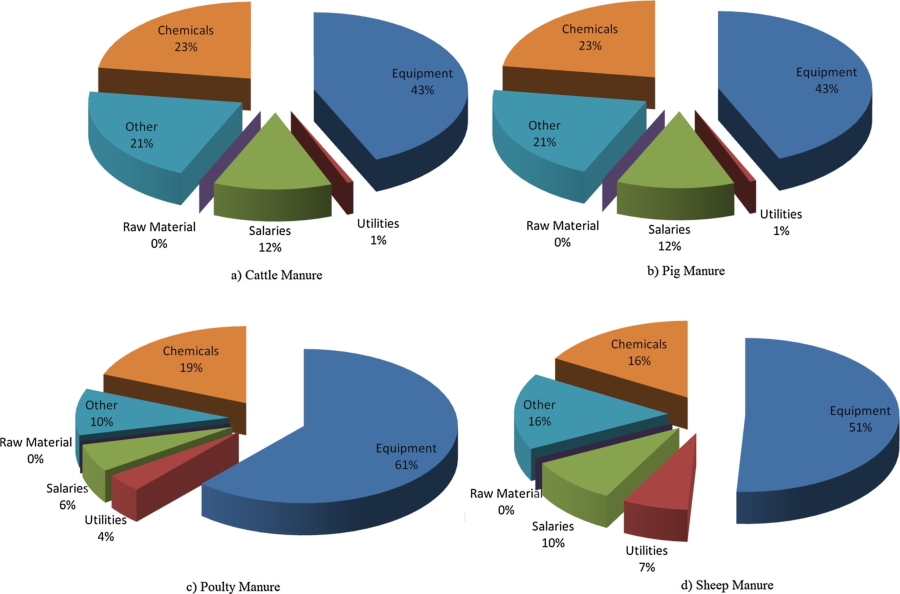
\includegraphics[width=0.9\linewidth, trim={0cm 0cm 0cm 0cm},clip]{gfx/Chapter2/Fig8.pdf} 
	\caption{Operation cost distribution for cattle, pig, poultry and sheep manure treatment.}
	\label{fig:OpCost}
\end{figure}

\subsection{Effect on the power, operating conditions and digestate treatment} \label{section:Effect}
The results obtained from the treatment of different manure streams show the influence of the manure composition in the amount produced and the composition of biogas and digestate obtained. Struvite production using FBR is the best choice for digestate treatment. This can be explained by the advantages in recovering nutrients in solid form since they can be easily transported and stored. Furthermore the material is highly concentrated in nutrients with a relatively high selling price. Biogas production is similar for cattle and pig manures, but is significantly higher in the poultry and sheep cases. The investment cost when processing cattle and pig manure is dominated by the digester, resulting in similar investment and production costs for facilities using either of the two types of manure. However, the higher concentration in organic matter in sheep and poultry manure does not only results in higher power production capacities, but the fact that the contribution to the cost of the turbines is also larger and so is the investment cost of these facilities. On the other hand, the electricity production cost is lower in the last two cases as result of the economies of scale between the investment cost and the biogas produced and the higher amount of struvite produced, with the extreme case of poultry manure where the struvite selling benefits are capable to cover the electricity production costs. Note that the availability of poultry and or sheep manure should be less that than for cattle and pig manure.


\section{Conclusions} \label{section:Conclusions}
In this work, we have designed optimal integrated facilities for the production of biogas-based electrical power and fertilizers from manure. Detailed equation based models for the anaerobic digestion, the Brayton and regenerative Rankine cycles and different technologies for digestate treatment have been developed. To solve the model a two-step procedure has been performed. First, the individual detailed models for each digestate treatment technology are used to formulate a MINLP model aiming at selecting the best configuration for that technology: the best precipitation agent, filter media, etc. In the second step, the best configuration of each technology has been implemented in the entire superstructure. Due to the fact that only one digestate processing technology is allowed and the highly non-linear nature of the model, surrogate models for the cost of each alternatives with a smooth approximations have been developed. For the optimal selection a detailed economic evaluation is performed. The results show that FBR technologies are preferred to recovery nutrients. Furthermore, in some cases this process can produce electricity at a competitive price (in case of poultry and sheep manure). The investment cost is highly dependent on the water and organic content of the manure type, ranging from 70 M EUR to 208 M EUR when a large energy production is possible and large gas and steam turbines are to be installed. However, for these cases of higher investment cost, the production cost of power is the most competitive due to the large production capacity. Biogas power plants show a wide range of values of power
per kW installed depending on the manure concentration. Competitive values of 4,000 EUR/kW for poultry manure are obtained, due to the highly concentrated manure, while large values of 25,000 EUR/kW installed are reported in case of the diluted cattle or pig manure.


\section*{Nomenclature}
\addcontentsline{toc}{section}{Nomenclature}

\vspace{-0.8cm}
\begingroup     
\let\clearpage\relax
%
 \newglossaryentry{set1}{type=SetsCh2,name={i},description={$\in \left\{ \text{P, N} \right\}$}}
 \newglossaryentry{set2}{type=SetsCh2,name={j},description={$\in \left\{ \text{filter media} \right\}$}}
 \newglossaryentry{set3}{type=SetsCh2,name={k},description={$\in \left\{ \text{TS, C, K} \right\}$}}
 \newglossaryentry{set4}{type=SetsCh2,name={a'},description={$\in \left\{\text{CH\textsubscript{4},  CO\textsubscript{2}, NH\textsubscript{3}, H\textsubscript{2}S, O\textsubscript{2}, N\textsubscript{2}}\right\}$}}
 \newglossaryentry{set5}{type=SetsCh2,name={a},description={$\in \left\{ \text{H\textsubscript{2}O, CH\textsubscript{4}, CO\textsubscript{2}, NH\textsubscript3, H\textsubscript{2}S, O\textsubscript{2}, N\textsubscript{2}} \right\}$}}
 \newglossaryentry{set6}{type=SetsCh2,name={d},description={$\in \left\{ \text{C, N\textsubscript{organic}, N\textsubscript{NH\textsubscript{3}}, P, K, H\textsubscript{2}O, Rest} \right\}$}}
 \newglossaryentry{set7}{type=SetsCh2,name={e},description={$\in \left\{ \text{CH\textsubscript{4}, NH\textsubscript{3}, H\textsubscript{2}S} \right\}$}}
 \newglossaryentry{set8}{type=SetsCh2,name={h},description={$\in \left\{ \text{CH\textsubscript{4}, CO\textsubscript{2}, O\textsubscript{2}, N\textsubscript{2}} \right\}$}}
 %
 \newglossaryentry{param1}{type=ParamCh2,name={$A_{specific}$},description={specific clarifier area (m\textsuperscript{2}/(ton·day))}}
 \newglossaryentry{param2}{type=ParamCh2,name={$A(i)$},description={Antoine $A$ coefficient for vapor pressure of component $i$}}
 \newglossaryentry{param3}{type=ParamCh2,name={$B(i)$},description={Antoine $B$ coefficient for vapor pressure of component $i$}}
 \newglossaryentry{param4}{type=ParamCh2,name={$C(i)$},description={Antoine $C$ coefficient for vapor pressure of component $i$}}
 \newglossaryentry{param5}{type=ParamCh2,name={$c_{p_{sat}}$},description={specific heat capacity of flue gas}}
 \newglossaryentry{param6}{type=ParamCh2,name={$d$},description={working days per year}}
 \newglossaryentry{param7}{type=ParamCh2,name={$d_{p}$},description={particle diameter (m)}}
 \newglossaryentry{param8}{type=ParamCh2,name={$k$},description={kinetic constant $\left( \text{s}^{-1}\right) $}}
 \newglossaryentry{param9}{type=ParamCh2,name={$IAP_{eq}$},description={ion activity product equilibrium}}
 \newglossaryentry{param10}{type=ParamCh2,name={$h$},description={working hours per day}}
 \newglossaryentry{param11}{type=ParamCh2,name={$HRT_{unit}$},description={hydraulic retention time of $unit$ (s)}}
 \newglossaryentry{param12}{type=ParamCh2,name={$MW_{component}$},description={molecular weight of $component$ (kg/kmol)}}
 \newglossaryentry{param13}{type=ParamCh2,name={$MeP_{ratio}$},description={metal/phosphorus molar ratio in coagulation process}}
 \newglossaryentry{param14}{type=ParamCh2,name={$Price_{component}$},description={price of $component$ (EUR/kg)}}
 \newglossaryentry{param15}{type=ParamCh2,name={$g$},description={gravity acceleration $\left(\text{m}^{2} / \text{s} \right)$}}
 \newglossaryentry{param16}{type=ParamCh2,name={$\kappa_{agitator}$},description={agitator specific power consumed (HP/1000 US gallon)}}
 \newglossaryentry{param17}{type=ParamCh2,name={$\varphi_j$},description={precipitation agent $j$ : total solids (mass ratio)}}
 \newglossaryentry{param18}{type=ParamCh2,name={$\eta_c$},description={compressors efficiency (0.85)}}
 \newglossaryentry{param19}{type=ParamCh2,name={$\eta_s$},description={isentropic efficiency (0.9)}}
 \newglossaryentry{param20}{type=ParamCh2,name={$\eta_i^j$},description={separation yield of componente $i$ in inprocess $j$}}
 \newglossaryentry{param21}{type=ParamCh2,name={$P_{atm}$},description={atmospheric pressure (1 bar)}}
 \newglossaryentry{param22}{type=ParamCh2,name={$T_{atm}$},description={room temperature (25 ºC)}}
 \newglossaryentry{param23}{type=ParamCh2,name={$R$},description={ideal gas constant (8.314 J/mol·K)}}
 \newglossaryentry{param24}{type=ParamCh2,name={$c_{p_{H_{2}O}}$},description={specific heat capacity of water (4.18 kJ/kg \textdegree C)}}
 %
 \newglossaryentry{var1}{type=VarCh2,name={$a_{technology}$},description={selection parameter which takes value 0 when $F_{design}^{technology}$is 0 and 1 if $F_{design}^{technology}$ is not equal to 0}}
 \newglossaryentry{var2}{type=VarCh2,name={$\alpha_{mf}$},description={parameter dependent of the number of phases in the FBR}}
 \newglossaryentry{var3}{type=VarCh2,name={$Ar_l$},description={Arquimedes number for liquid}}
 \newglossaryentry{var4}{type=VarCh2,name={$A_unit$},description={area of unit $\left( \text{m}^2 \right)$}}
 \newglossaryentry{var5}{type=VarCh2,name={$Benefits_{technology}$},description={benefits or losses obtained with $technology$}}
 \newglossaryentry{var6}{type=VarCh2,name={$C:N$},description={carbon to nitrogen molar ratio}}
 \newglossaryentry{var7}{type=VarCh2,name={$C_{eq}$},description={equilibrium concentration (kmol/m\textsuperscript{3})}}
 \newglossaryentry{var8}{type=VarCh2,name={$C_0$},description={initial concentration (kmol/m\textsuperscript{3})}}
 \newglossaryentry{var9}{type=VarCh2,name={$Cost_{unit}$},description={cost of $unit$}}
 \newglossaryentry{var10}{type=VarCh2,name={$C_{component}^{unit}$},description={concentration of $component$ in the $unit$ inlet stream $\left(\text{kg\textsubscript{component}} / \text{kg\textsubscript{total}} \right) $}}
 \newglossaryentry{var11}{type=VarCh2,name={$ChemC_technology$},description={cost of chemicals for $technology$}}
 \newglossaryentry{var12}{type=VarCh2,name={$D_{unit}$},description={diameter of $unit$}}
 \newglossaryentry{var13}{type=VarCh2,name={$e_{unit}$},description={thickness of $unit$}}
 \newglossaryentry{var14}{type=VarCh2,name={$Ec_{j}\left( T \right)$},description={equilibrium constant of component $j$ at temperature T}}
 \newglossaryentry{var15}{type=VarCh2,name={$F_{component}^{unit}$},description={mass flow of $component$ in the $unit$ inlet stream (kg/s)}}
 \newglossaryentry{var16}{type=VarCh2,name={$F_{max}^{unit}$},description={maximum mass inlet flow admitted by a single unit (kg/s)}}
 \newglossaryentry{var17}{type=VarCh2,name={$F_{design}^{unit}$},description={mass inlet flow used in the design of $unit$ (kg/s)}}
 \newglossaryentry{var18}{type=VarCh2,name={$FC_{technology}$},description={fixed cost of $technology$}}
 \newglossaryentry{var19}{type=VarCh2,name={$F_{total}^{recovered}$},description={recovered matter total mass flow (kg/s)}}
 \newglossaryentry{var20}{type=VarCh2,name={$F^{unit,unit1}$},description={mass flow from stream from $unit$ to $unit1$ (kg/s)}}
 \newglossaryentry{var21}{type=VarCh2,name={$fc_{j}^{unit,unit1}$},description={mass flow of component $j$ from $unit$ to $unit1$ (kg/s)}}
 \newglossaryentry{var22}{type=VarCh2,name={$H_{b}^{unit,unit1)}$},description={enthalpy of the stream at state b from $unit$ to $unit1$ (kJ/kg)}}
 \newglossaryentry{var23}{type=VarCh2,name={$H_{steam (isoentropy)}$},description={isentropic expansion enthalpy of steam (kJ/kg)}}
 \newglossaryentry{var24}{type=VarCh2,name={$l_{j-i}$},description={molar fraction of component $j$ in the liquid phase of equilibrium system $i$}}
 \newglossaryentry{var25}{type=VarCh2,name={$K_{index}$},description={potassium index of fertilizer}}
 \newglossaryentry{var26}{type=VarCh2,name={$L_{unit}$},description={length of $unit$}}
 \newglossaryentry{var27}{type=VarCh2,name={$N_{NH_{3}}$},description={nitrogen contained in ammonia}}
 \newglossaryentry{var28}{type=VarCh2,name={$N_{org}$},description={nitrogen contained in organic matter}}
 \newglossaryentry{var29}{type=VarCh2,name={$n_{unit}$},description={number of units used in the process}}
 \newglossaryentry{var30}{type=VarCh2,name={$n_{(unit,unit1)}$},description={total mol flow from stream from $unit$ to $unit1$ (kmol/s)}}
 \newglossaryentry{var31}{type=VarCh2,name={$N_{index}$},description={nitrogen index of fertilizer}}
 \newglossaryentry{var32}{type=VarCh2,name={$P_{in/compressor}$},description={inlet pressure to compressor (bar)}}
 \newglossaryentry{var33}{type=VarCh2,name={$P_{out/compressor}$},description={outlet pressure of compressor (bar)}}
 \newglossaryentry{var34}{type=VarCh2,name={$P_j^{*} \left( T \right)$},description={saturation pressure of pure component $j$ at temperature T (bar)}}
 \newglossaryentry{var35}{type=VarCh2,name={$P_v$},description={vapor pressure (bar)}}
 \newglossaryentry{var36}{type=VarCh2,name={$P_{index}$},description={phosphorous index of fertilizer}}
 \newglossaryentry{var37}{type=VarCh2,name={$p_{turb,i}$},description={inlet pressure to body $i$ in the turbine (bar)}}
 \newglossaryentry{var38}{type=VarCh2,name={$P_{unit}$},description={power of unit}}
 \newglossaryentry{var39}{type=VarCh2,name={$Q_{(unit)}$},description={heat exchanged in $unit$ (kW)}}
 \newglossaryentry{var40}{type=VarCh2,name={$R_{C-N/k}$},description={carbon to nitrogen ratio in $k$}}
 \newglossaryentry{var41}{type=VarCh2,name={$R_{C-N/fertilizer}$},description={carbon to nitrogen ratio in fertilizer}}
 \newglossaryentry{var42}{type=VarCh2,name={$R_{V-F/i}$},description={rate of evaporation in equilibrium system $i$}}
 \newglossaryentry{var43}{type=VarCh2,name={$Rest$},description={rest of the elements contained in the biomass}}
 \newglossaryentry{var44}{type=VarCh2,name={$Re_{l,mf}$},description={Reynolds number for liquid in minimum fluidization conditions}}
 \newglossaryentry{var45}{type=VarCh2,name={$s_{b,(unit,unit1)}$},description={entropy the stream at the state $b$ for the stream from $unit$ to $unit1$ (kJ/kg·K)}}
 \newglossaryentry{var46}{type=VarCh2,name={$T_{turb,i, min}^{*}$},description={saturated temperature at exit of body $i$ (\textdegree C)}}
 \newglossaryentry{var47}{type=VarCh2,name={$T_{(unit,unit1)}$},description={temperature of the stream from $unit$ to $unit1$ (\textdegree C)}}
 \newglossaryentry{var48}{type=VarCh2,name={$T_{bubble/i}$},description={bubble point temperature of equilibrium system $i$ (\textdegree C)}}
 \newglossaryentry{var49}{type=VarCh2,name={$T_{m/i}$},description={average temperature in equilibrium system $i$ (\textdegree C)}}
 \newglossaryentry{var50}{type=VarCh2,name={$T_{in/compressor}$},description={inlet temperature to compressor (\textdegree C)}}
 \newglossaryentry{var51}{type=VarCh2,name={$T_{out/compressor}$},description={outlet temperature of compressor (\textdegree C)}}
 \newglossaryentry{var52}{type=VarCh2,name={$t$},description={time (s)}}
 \newglossaryentry{var53}{type=VarCh2,name={$u_t$},description={terminal velocity (m/s)}}
 \newglossaryentry{var54}{type=VarCh2,name={$u_0$},description={fluid velocity (m/s)}}
 \newglossaryentry{var55}{type=VarCh2,name={$u_{mf}$},description={minimum fluidization velocity (m/s)}}
 \newglossaryentry{var56}{type=VarCh2,name={$v_{j-i}$},description={molar fraction of component $j$ in the vapor phase of equilibrium system $i$}}
 \newglossaryentry{var57}{type=VarCh2,name={$V_{biogas,k}$},description={biogas volume produced per unit of volatile solids (VS) associated to waste $k$ (m\textsuperscript{3}\textsubscript{biogas}/kg\textsubscript{VS/k})}}
 \newglossaryentry{var58}{type=VarCh2,name={$V_{unit}$},description={volume of $unit$}}
 \newglossaryentry{var59}{type=VarCh2,name={$W_{unit}$},description={weight of $unit$}}
 \newglossaryentry{var60}{type=VarCh2,name={$w^\prime_{DM/k}$},description={dry mass fraction of $k$ (kg\textsubscript{DM/k}/kg)}}
 \newglossaryentry{var61}{type=VarCh2,name={$w^\prime_{VS/k}$},description={dry mass fraction of volatile solids out of the dry mass of $k$ (kg\textsubscript{VS/k}/kg\textsubscript{DM/k})}}
 \newglossaryentry{var62}{type=VarCh2,name={$w^\prime_{C/k}$},description={dry mass fraction of C in $k$ (kg\textsubscript{C/k}/kg\textsubscript{DM/k})}}
 \newglossaryentry{var63}{type=VarCh2,name={$w^\prime_{NH_{3}/k}$},description={dry mass fraction of NH\textsubscript{3} in $k$ (kg\textsubscript{NH\textsubscript{3}/k}/kg\textsubscript{DM/k})}}
 \newglossaryentry{var64}{type=VarCh2,name={$w^\prime_{N_{org}/k}$},description={dry mass fraction of N\textsubscript{org} in $k$ (kg\textsubscript{N\textsubscript{org}/k}/kg\textsubscript{DM/k})}}
 \newglossaryentry{var65}{type=VarCh2,name={$w^\prime_{P/k}$},description={dry mass fraction of P in $k$ (kg\textsubscript{P/k}/\textsubscript{DM/k})}}
 \newglossaryentry{var66}{type=VarCh2,name={$w^\prime_{K/k}$},description={dry mass fraction of K in $k$ (kg\textsubscript{K/k}/\textsubscript{DM/k})}}
 \newglossaryentry{var67}{type=VarCh2,name={$w^\prime_{Rest/k}$},description={dry mass fraction of the rest of the elements contained in $k$ (kg\textsubscript{Rest/k}/kg\textsubscript{DM/k})}}
 \newglossaryentry{var68}{type=VarCh2,name={$W_{unit}$},description={power produced or consumed in $unit$ (kW)}}
 \newglossaryentry{var69}{type=VarCh2,name={$w^\prime_{Rest/k}$},description={dry mass fraction of the rest of the elements contained in $k$ (kg\textsubscript{Rest/k}/kg\textsubscript{DM/k})}}
 \newglossaryentry{var70}{type=VarCh2,name={$x_{a/biogas}$},description={mass fraction of component $a$ in the biogas}}
 \newglossaryentry{var71}{type=VarCh2,name={$y^j$},description={binary variable to evaluate the element $j$}}
 \newglossaryentry{var72}{type=VarCh2,name={$y_{biogas}$},description={specific saturated moisture of biogas}}
 \newglossaryentry{var73}{type=VarCh2,name={$w^\prime_{Rest/k}$},description={dry mass fraction of the rest of the elements contained in $k$ (kg\textsubscript{Rest/k}/kg\textsubscript{DM/k})}}
 \newglossaryentry{var74}{type=VarCh2,name={$Y_{a', biogas-dry}$},description={molar fraction of component a in the dry biogas}}
 \newglossaryentry{var75}{type=VarCh2,name={$\Delta H_{reaction(bioreactor)}$},description={reaction heat of anaerobic digestion (kW)}}
 \newglossaryentry{var76}{type=VarCh2,name={$\Delta H_{comb, k}$},description={heat of combustion of component $k$ (kW)}}
 \newglossaryentry{var77}{type=VarCh2,name={$\Delta H_{comb, e}$},description={heat of combustion of component $e$ (kW)}}
 \newglossaryentry{var78}{type=VarCh2,name={$\Delta H_{comb, digestate-dry}$},description={heat of combustion of dry digestate (kW)}}
 \newglossaryentry{var79}{type=VarCh2,name={$\Delta H_{f, h} \left( T \right) $},description={heat of formation of component $h$ at temperature T (kW)}}
 \newglossaryentry{var80}{type=VarCh2,name={$Z$},description={objective function}}
 \newglossaryentry{var81}{type=VarCh2,name={$\rho_{component}$},description={density of $component$ (kg/m\textsuperscript{3})}}
 \newglossaryentry{var82}{type=VarCh2,name={$\mu_{component}$},description={viscosity of component (kg/(m·s))}}

%
\glsaddall
%**************************************************************
%This is for horizontal spacing between acronym and description
\setlength\LTleft{0pt}
\setlength\LTright{0pt}
\setlength\glsdescwidth{0.8\hsize}
%**************************************************************
%**************************************************************
%This is for vertical spacing between title and entries
\renewcommand*{\glossarypreamble}{\vspace{-0.8cm}}
%**************************************************************
\printglossary[type=SetsCh2, style=long]
\vspace{10pt}
\printglossary[type=ParamCh2, style=long]
\vspace{10pt}
\printglossary[type=VarCh2, style=long]
%\printglossaries
\endgroup

\section*{Acknowledgments} \label{section:AcknowledgmentsPaper1}
\addcontentsline{toc}{section}{Acknowledgments}
We acknowledge funding from the National Science Foundation (under grant CBET-1604374) and MINECO (under grant DPI2015-67341-C2-1-R) and E.M. also acknowledges an undergraduate research grant.

\section*{Bibliography}
\addcontentsline{toc}{section}{Bibliography}

\printbibliography[heading=none]
\end{refsection}
%\printbibliography[heading=none]
